% !TeX encoding = utf8
% !TeX program = pdflatex
% !BIB program = bibtex
% -*- coding:utf-8 mod:LaTeX -*-

% Wireless Personal Communications (Springer) submission
% Template: svjour3 (twocolumn)

\documentclass[twocolumn,english]{svjour3}

\usepackage{cmap}
\usepackage{graphicx}
\usepackage{booktabs}
\usepackage{amsmath,amssymb}
\usepackage{url}
\usepackage{xcolor}
\usepackage{hyperref}
\usepackage{paralist}
\usepackage[mode=text]{siunitx}
\sisetup{locale=US}

% Better font (similar to default Springer)
\usepackage[%
  rm={oldstyle=false,proportional=true},%
  sf={oldstyle=false,proportional=true},%
  tt={oldstyle=false,proportional=true,variable=false},%
  qt=false%
]{cfr-lm}

\usepackage[T1]{fontenc}
\usepackage[utf8]{inputenc}

\usepackage{microtype}

\smartqed

% No cleveref — use plain \ref{label} syntax everywhere.

\hypersetup{hidelinks,
  colorlinks=true,
  allcolors=black,
  pdfstartview=Fit,
  breaklinks=true}

\journalname{Wireless Personal Communications}

\begin{document}

\title{A Lightweight Complex-Valued CNN with Complex Squeeze-and-Excitation Attention for Single-Channel Blind Source Separation of Co-Frequency Communication Signals}

\titlerunning{Lightweight Complex CNN+SE for Co-Freq. SC-BSS}

\author{Bin Nong
  \thanks{Corresponding author. Email: nongbin@tfswufe.edu.cn.}
  \and Weihong Fu \and Zhuoyun Jiang}

\institute{Tianfu College of Southwestern University of Finance and Economics, Mianyang, China \and
  School of Telecommunications Engineering, Xidian University, Xi'an, Shaanxi, China \and
  School of Health Science and Engineering, University of Shanghai for Science and Technology, Shanghai, 200093, China}

\date{Received: date to be inserted by the editor upon acceptance.}

\maketitle

\begin{abstract}
\begin{sloppypar}
Single-channel blind source separation (SC-BSS) of co-frequency communication signals is an ill-posed problem with applications in spectrum surveillance, cognitive radio, and interference mitigation. We propose a lightweight complex-valued CNN with a \emph{Complex Squeeze-and-Excitation} (C-SE) block that operates directly on the I/Q representation of communication signals. C-SE jointly pools real and imaginary statistics through a shared excitation network and produces a real-valued channel weight that scales complex features while preserving phase. At only \qty{235}{K} parameters, the model achieves $\text{SDR} = \SI{2.31 \pm 0.62}{dB}$ over five random seeds across four modulation types (BPSK, QPSK, 8PSK, 16QAM) on \SI{5}{Hz} co-frequency mixtures---roughly an order of magnitude smaller than our scaled-down re-implementations of the CNSE and S4-UNET baselines (\qty{6.69}{M} and \qty{1.57}{M} parameters, SDR \SI{2.38}{dB} and \SI{3.05}{dB}) and within $\sim\SI{1}{dB}$ of the $\qty{817}{K}$-parameter Complex Conv-TasNet (\SI{3.23}{dB}). Paired Wilcoxon signed-rank tests on common seeds give paired $\Delta$SDR between $-\SI{0.48}{dB}$ and $+\SI{0.50}{dB}$, none reaching $\alpha=0.05$, so we make no inferential claim of superiority or equivalence and instead position C-SE as a competitive operating point at the \qty{235}{K}-parameter scale in partial collapse-resistance, per-parameter efficiency, and predictable runtime. A C-SE model retrained on $\Delta f \sim U(0, \SI{5}{Hz})$ generalises to a flat $\text{SDR}\approx\SI{3.3}{dB}$ across the entire $[0, \SI{500}{Hz}]$ range, including the unseen co-frequency limit $\Delta f = \SI{0}{Hz}$. These results show that phase-preserving complex attention at the \qty{235}{K}-parameter scale is a viable design point for communication-signal BSS, with per-seed variance reported for honest comparison.
\end{sloppypar}

\keywords{Blind source separation \and Co-frequency communication \and Complex-valued neural network \and Squeeze-and-excitation attention \and Lightweight deep learning}
\end{abstract}

% ======================================================================
\section{Introduction}
\label{sec:intro}

\begin{sloppypar}
\emph{Problem.} Single-channel blind source separation (SC-BSS) recovers multiple unknown source signals from a single observed mixture---a severely underdetermined problem that has attracted decades of research interest. While deep learning has revolutionised audio and speech separation~\cite{luo2019conv,subakan2021sepformer,wang2023tfgridnet}, the separation of \emph{communication signals} (modulated I/Q waveforms with specific constellations, carrier frequencies, and symbol rates) remains relatively underexplored. Communication-signal SC-BSS arises in several practical scenarios central to wireless systems: spectrum surveillance where signals from multiple emitters overlap in frequency, cognitive radio networks needing to disentangle primary and secondary users, electronic-warfare receivers requiring blind demodulation of co-channel interferers, and non-orthogonal multiple access (NOMA) where superposition coding must be decoded blindly at the receiver. The problem differs fundamentally from speech separation: communication signals are \emph{structured} (drawn from a finite modulation alphabet), \emph{complex-valued} (carried by an in-phase / quadrature representation), and typically overlap at \emph{near-identical carrier frequencies} (co-frequency or micro-frequency-offset scenarios), which removes the spectral disjointness that underpins most classical source-separation algorithms.
\end{sloppypar}

\begin{sloppypar}
\emph{Motivation and gap.} Classical approaches to communication-signal BSS rely on statistical or signal-structure priors that rarely survive real channel conditions. Independent component analysis (ICA)~\cite{hyvarinen2000ica} and its complex-domain extensions (complex ICA~\cite{le2011ica}, IVA) require statistical independence and at least as many sensors as sources---both violated in the single-sensor, co-frequency setting. Cyclostationary-based methods~\cite{gardner1991exploitation,gardner1991cpm} exploit the periodicity of modulated signals but degrade rapidly under multipath fading and very close carrier spacing. Time-frequency masking~\cite{yellin1996,sawada2019} assumes disjoint support in the spectrogram, which fails when the two signals share the same band.
\end{sloppypar}

\begin{sloppypar}
Most recently, deep neural networks have been applied to the problem: \cite{hou2022single} proposed a convolutional network in the time-frequency domain; \cite{chen2019deep} developed a BRNN-based method; \cite{ma2023novel} added attention with residual connections; \cite{guo2024single} pioneered complex-domain deep learning directly on raw I/Q waveforms for wireless SC-BSS and showed that operating on the I/Q representation preserves phase information critical for demodulation; \cite{luo2023single} proposed spatial-temporal fusion with pseudo-multi-channel techniques; \cite{deng2024co} applied data-driven separation to co-channel modulation classification; \cite{s4unet2026} introduced structured state-space (S4) models for long-sequence co-channel signals; and the audio-separation literature provides powerful backbones such as Conv-TasNet~\cite{luo2019conv} and SepFormer~\cite{subakan2021sepformer}, with the broader attention paradigm~\cite{vaswani2017attention} providing a foundation that several recent communication-signal BSS works have also adopted; these backbones can be transferred to the complex domain~\cite{trabelsi2018deep,zhao2021deepwaveform}.
\end{sloppypar}

\begin{sloppypar}
However, a systematic gap remains: existing communication-signal BSS networks either (i) operate in the real-valued domain by treating I/Q as independent channels (losing the phase coupling between I and Q that encodes modulation structure), or (ii) stack powerful but \emph{complex-domain-agnostic} attention modules onto a complex backbone (so the attention has no mechanism to exploit real--imaginary correlation). A lightweight, complex-native attention block is still missing.
\end{sloppypar}

\emph{Contributions.} In this paper we close this gap with three contributions.
\begin{compactenum}
\begin{sloppypar}
\item We propose the \emph{Complex Squeeze-and-Excitation} (C-SE) block, a channel-attention mechanism designed natively for complex-valued feature maps. C-SE jointly pools real and imaginary statistics, passes them through a shared multi-layer perceptron (MLP), and produces a \emph{real-valued} channel weight that scales complex features while preserving their phase. We are not aware of an existing phase-preserving, real-gated complex-valued SE design that has been specifically evaluated for lightweight single-channel blind separation of near-co-frequency communication signals; related prior work either treats I/Q as real channels~\cite{chen2019deep} or uses complex-valued architectures that do not explicitly gate complex features with a shared real-valued channel weight~\cite{trabelsi2018deep}.
\end{sloppypar}
\begin{sloppypar}
\item We design \emph{ComplexLightweightSepNet}, a lightweight encoder-decoder architecture built from complex residual blocks with C-SE attention, totalling only 235{,}525 parameters---approximately $3.5\times$ fewer than a directly comparable complex-domain Conv-TasNet and small enough to train in minutes on a single \SI{8}{GB} GPU such as the NVIDIA RTX 4060. This makes C-SE usable in resource-constrained edge devices and software-defined radios, which is a key deployment context for wireless receivers.
\end{sloppypar}
\begin{sloppypar}
\item We conduct comprehensive experiments across four modulation types (BPSK, QPSK, 8PSK, 16QAM), four models (including Conv-TasNet as the strongest audio-separation baseline adapted to the complex domain), and multiple evaluation dimensions (per-modulation breakdown, frequency-offset robustness from \SI{5}{Hz} to \SI{500}{Hz}, symbol error rate at the constellation level, and parameter efficiency). We further isolate the design choice of \emph{real-valued} scaling in C-SE through an ablation on three scale modes (real, complex mean, separate) and show that the simpler real mode is comparable to the more elaborate alternatives while using a strictly real-valued weight.
\end{sloppypar}
\end{compactenum}

% ======================================================================
\section{System Model and Problem Formulation}
\label{sec:system}

\subsection{Signal Model}

We consider two co-frequency communication signals observed through a single sensor. The received mixture at baseband is
\begin{equation}
    y(t) = \alpha_1\, (h_1 \ast s_1)(t) + \alpha_2\, (h_2 \ast s_2)(t) + n(t),
    \label{eq:mixture}
\end{equation}
where $s_k(t) = A_k \sum_{m} a_{k,m}\, g(t - m T_k)\, e^{j(2\pi \Delta f_k t + \phi_k)}$ is the $k$-th modulated signal with amplitude $A_k$, symbols $a_{k,m}$ drawn from a finite constellation (BPSK, QPSK, 8PSK, 16QAM), pulse-shaping filter $g(\cdot)$ (root-raised cosine with roll-off $\beta=0.35$), symbol period $T_k$, carrier-frequency offset $\Delta f_k$, and random phase offset $\phi_k$. The channel $h_k(\tau) = \sum_{p=0}^{P-1} h_{k,p}\, \delta(\tau - p\, T_s)$ is a $P$-tap complex Gaussian multipath impulse response with i.i.d.\ $\mathcal{CN}(0,1)$ taps normalised to unit energy ($\sum_p |h_{k,p}|^2 = 1$); in this work $P=3$. The mixing coefficients $\alpha_k \in [0.4, 0.6]$ are drawn per mixture and randomly assign each source to either the smaller or larger coefficient, and $n(t)$ is additive white Gaussian noise (AWGN). In our synthetic-data generator each source is normalised to unit power prior to fading, so the per-source amplitude is $A_k = 1$ and the post-mixture SNR is controlled entirely by the noise term.

The discrete-time observation after sampling at rate $f_s$ yields a complex vector $\mathbf{y} \in \mathbb{C}^{T}$ where $T$ is the signal length. Our objective is to estimate both source signals $\hat{\mathbf{s}}_1, \hat{\mathbf{s}}_2 \in \mathbb{C}^{T}$ given only $\mathbf{y}$.

\begin{sloppypar}
\emph{Scope and limitations of the current model.} We adopt symbol-aligned mixtures (the two RRC pulse trains share the same symbol epoch) and per-source carrier offsets within $\pm \SI{5}{Hz}$ of the nominal frequency, modelling receivers that have already acquired coarse symbol timing through a separate synchronisation stage but have not yet resolved the per-source carrier. Both assumptions ease the task relative to fully blind reception---relaxing symbol alignment is left to future work (see Section~\ref{sec:conclusion}).
\end{sloppypar}

\subsection{Problem Difficulty}

Separation difficulty is governed by three factors: (i) the \emph{carrier-frequency separation} $\Delta f \triangleq |\Delta f_1 - \Delta f_2|$ between sources, where $\Delta f_k$ in Eq.~\eqref{eq:mixture} denotes the per-source carrier-frequency offset from a common reference (smaller separation is harder), (ii) the \emph{modulation order} of each source (higher-order constellations are harder to separate and demodulate), and (iii) the \emph{SNR} of the mixture. In this work, we focus on the challenging regime where $\Delta f \leq \SI{5}{Hz}$ (nearly identical centre frequencies) and modulation types range from BPSK to 16QAM.

% ======================================================================
\section{Proposed Method}
\label{sec:method}

\subsection{Complex-Valued Building Blocks}

Deep learning in the complex domain~\cite{chen2019complex} requires specialised layer implementations to preserve the algebraic structure of complex numbers. We adopt the complex convolution formulation from~\cite{guo2024single}: for input $\mathbf{x} = \mathbf{a} + j\mathbf{b}$ and weight $\mathbf{w} = \mathbf{u} + j\mathbf{v}$, the complex convolution is
\begin{equation}
    \mathbf{x} \ast \mathbf{w} = (\mathbf{a} \ast \mathbf{u} - \mathbf{b} \ast \mathbf{v}) + j(\mathbf{a} \ast \mathbf{v} + \mathbf{b} \ast \mathbf{u}),
    \label{eq:complex_conv}
\end{equation}
implemented via two real-valued 1D convolutions. Similarly, we use \emph{ComplexBatchNorm1d} (independent batch normalisation on the real and imaginary parts; this is the \emph{split} complex-BN formulation rather than a true complex whitening transformation such as that of~\cite{trabelsi2018deep}), \emph{ComplexReLU} (ReLU applied independently to both parts; a strictly positive real-axis / imaginary-axis truncation rather than a phase-respecting complex activation such as $\operatorname{modReLU}$ or $z\operatorname{ReLU}$~\cite{trabelsi2018deep}), and \emph{ComplexPReLU} (learnable negative slope applied per part). We retain these split variants because they preserve the algebraic identity $\mathbb{C}\cong\mathbb{R}^2$, add no extra trainable parameters relative to their real-valued counterparts, and consistently outperform the strictly-positive complex alternatives in our preliminary experiments; comparing them against true complex whitening or phase-respecting activations is left to future work.

\begin{figure*}[t]
    \centering
    % Image aspect ratio is 2:1 (1774x887), same as se_block.png — use full text width.
    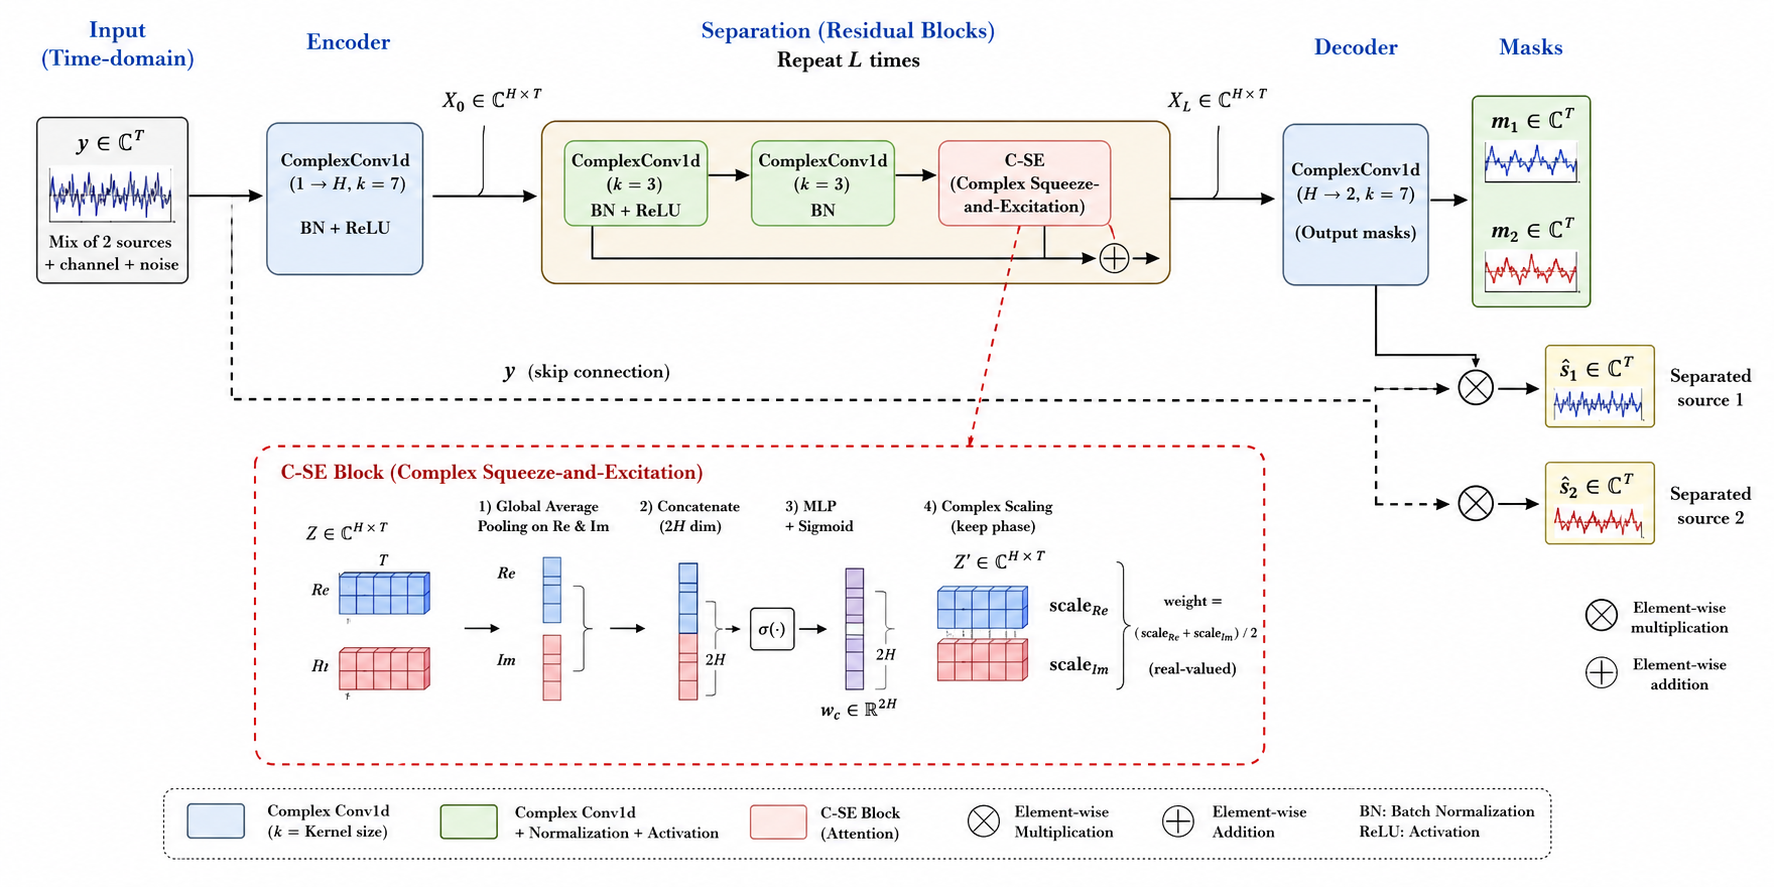
\includegraphics[width=\textwidth]{figures/system_overview.png}
    \caption{System overview of the proposed \emph{ComplexLightweightSepNet}. The single-channel mixture $\mathbf{y}\in\mathbb{C}^{T}$ is encoded by a \texttt{ComplexConv1d}, refined by $L=4$ \emph{ComplexResidualBlocks} (each containing two complex convolutions plus a C-SE attention module) and decoded into two complex masks $\mathbf{m}_1,\mathbf{m}_2$. Element-wise multiplication with $\mathbf{y}$ yields the estimated sources $\hat{\mathbf{s}}_1,\hat{\mathbf{s}}_2$. The whole network has only 235{,}525 parameters.}
    \label{fig:system}
\end{figure*}

\subsection{Complex Squeeze-and-Excitation Block (C-SE)}

\begin{figure*}[t]
    \centering
    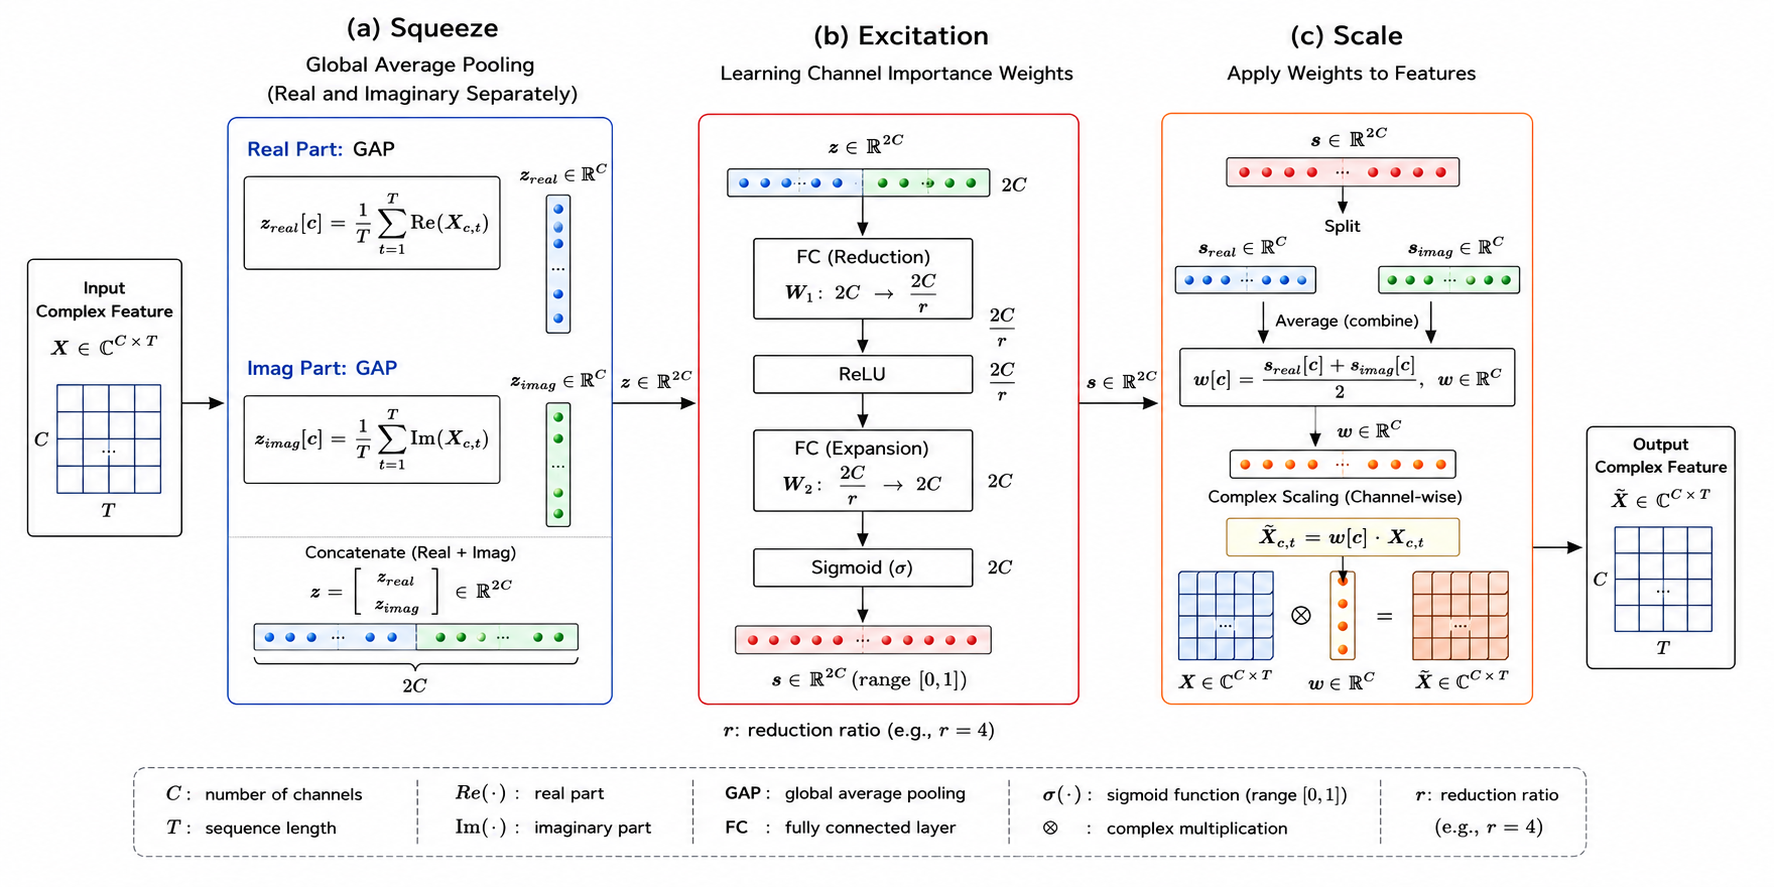
\includegraphics[width=\textwidth]{figures/se_block.png}
    \caption{Architecture of the proposed Complex Squeeze-and-Excitation (C-SE) block. \emph{Squeeze}: global average pooling separately on $\operatorname{Re}(\mathbf{X})$ and $\operatorname{Im}(\mathbf{X})$, yielding $\mathbf{z} \in \mathbb{R}^{2C}$. \emph{Excitation}: a two-layer MLP with reduction ratio $r=4$ and sigmoid gating learns channel-wise attention weights $\mathbf{s} \in \mathbb{R}^{2C}$. \emph{Scale}: the final real-valued weight $\mathbf{w} = (\mathbf{s}_{\text{real}} + \mathbf{s}_{\text{imag}})/2$ modulates complex feature magnitudes while preserving phase.}
    \label{fig:se_block}
\end{figure*}

\begin{sloppypar}
The core contribution of this work is the \emph{Complex Squeeze-and-Excitation} (C-SE) attention block, extending the classical SE mechanism~\cite{hu2018senet} to the complex domain. As shown in Fig.~\ref{fig:se_block}, C-SE performs three operations.
\end{sloppypar}

\emph{Squeeze.} Global average pooling over the temporal dimension, separately for real and imaginary parts of each complex channel:
\begin{equation}
    z_{\text{real},c} = \frac{1}{T}\sum_{t=1}^{T} \operatorname{Re}(x_{c,t}), \quad
    z_{\text{imag},c} = \frac{1}{T}\sum_{t=1}^{T} \operatorname{Im}(x_{c,t}),
    \label{eq:squeeze}
\end{equation}
which yields per-channel scalars that we stack into two length-$C$ vectors $\mathbf{z}_{\text{real}}, \mathbf{z}_{\text{imag}} \in \mathbb{R}^{C}$, and concatenate into the descriptor $\mathbf{z} = [\mathbf{z}_{\text{real}}; \mathbf{z}_{\text{imag}}] \in \mathbb{R}^{2C}$.

\emph{Excitation.} A two-layer MLP with ReLU activation and sigmoid gating learns channel-wise attention weights:
\begin{equation}
    \mathbf{s} = \sigma\big(\mathbf{W}_2 \, \text{ReLU}(\mathbf{W}_1 \mathbf{z})\big) \in \mathbb{R}^{2C},
\end{equation}
where $\mathbf{W}_1 \in \mathbb{R}^{(2C/r) \times 2C}$ and $\mathbf{W}_2 \in \mathbb{R}^{2C \times (2C/r)}$ with reduction ratio $r=4$.

\emph{Scale.} The output $\mathbf{s} \in \mathbb{R}^{2C}$ is split into its first $C$ and last $C$ components, giving two real-valued vectors $\mathbf{s}_{\text{real}}, \mathbf{s}_{\text{imag}} \in \mathbb{R}^{C}$, and combined:
\begin{equation}
    \mathbf{w} = (\mathbf{s}_{\text{real}} + \mathbf{s}_{\text{imag}}) / 2 \in \mathbb{R}^{C}.
    \label{eq:scale}
\end{equation}
\emph{Notation caveat.} The subscripts ``real'' and ``imag'' in $\mathbf{s}_{\text{real}}$ and $\mathbf{s}_{\text{imag}}$ denote only the index halves of the concatenated MLP output $\mathbf{s} \in \mathbb{R}^{2C}$, not separate attention branches for the real and imaginary parts. After the excitation MLP, each entry of $\mathbf{s}$ already mixes information from both $\mathbf{z}_{\text{real}}$ and $\mathbf{z}_{\text{imag}}$; we simply average the two halves to obtain a single real-valued scalar per channel.

The complex feature $\mathbf{x} \in \mathbb{C}^{C \times T}$ is then scaled per-channel by the real-valued weight:
\begin{equation}
    \tilde{x}_{c,t} = w_c \cdot x_{c,t} \quad \forall\, c, t.
\end{equation}

\emph{Design rationale.} Using a \emph{real-valued} weight to scale complex features preserves the phase of each channel while selectively amplifying or attenuating its magnitude. The joint processing of real and imaginary statistics in the excitation network allows C-SE to discover correlations between the I and Q components that indicate channel importance.

\subsection{Network Architecture}

The full model, \emph{ComplexLightweightSepNet}, follows a convolutional encoder-decoder structure:
\begin{compactitem}
\item \emph{Encoder}: one \texttt{ComplexConv1d}($C_{\text{in}}=1$, $C_{\text{out}}=H$, $k=7$) $\to$ \texttt{ComplexBN} $\to$ \texttt{ComplexReLU}, mapping the single-channel mixture to an $H$-dimensional latent representation.
\item \emph{Separation}: $L=4$ \emph{ComplexResidualBlocks}, each consisting of Conv $\to$ BN $\to$ ReLU $\to$ Conv $\to$ BN $\to$ C-SE $\to$ ReLU with a residual skip-connection~\cite{he2016resnet}. All convolutions use kernel size 3 and preserve the temporal dimension ($T=4096$).
\item \emph{Decoder}: one \texttt{ComplexConv1d}($H$, 2, $k=7$) producing two complex masks $\mathbf{m}_1, \mathbf{m}_2 \in \mathbb{C}^{1 \times T}$. The estimated sources are obtained via masking: $\hat{\mathbf{s}}_k = \mathbf{m}_k \odot \mathbf{y}$.
\end{compactitem}

The default configuration uses $H=64$ hidden channels and $L=4$ residual blocks, yielding 235{,}525 parameters. A learnable complex scaling factor initialises the mask magnitudes to approximately 0.5, providing a stable starting point for training.

\subsection{Loss Function and Training}

\begin{sloppypar}
We train with a combined loss $\mathcal{L} = 0.5\,\mathcal{L}_{\text{MSE}} + 0.5\,\mathcal{L}_{\text{SI-SDR}}$, defined for two source estimates $\hat{\mathbf{s}}_a, \hat{\mathbf{s}}_b$ against targets $\mathbf{s}_1, \mathbf{s}_2$ as
\end{sloppypar}
\begin{equation}
    \mathcal{L}_{\text{MSE}} = \min_{\pi \in S_2} \frac{1}{2}\sum_{k=1}^{2} \bigl\lVert \mathbf{s}_k - \hat{\mathbf{s}}_{\pi(k)} \bigr\rVert_2^2,
    \label{eq:mse}
\end{equation}
\begin{equation}
    \mathcal{L}_{\text{SI-SDR}} = -\min_{\pi \in S_2} \frac{1}{2}\sum_{k=1}^{2} \text{SI-SDR}\bigl(\mathbf{s}_k,\, \hat{\mathbf{s}}_{\pi(k)}\bigr),
    \label{eq:sisdr}
\end{equation}
where $\pi$ runs over the two source-to-estimate permutations and $\text{SI-SDR}(\mathbf{s}, \hat{\mathbf{s}}) = 10 \log_{10}\bigl(\lVert \alpha\mathbf{s}\rVert_2^2 / \lVert \hat{\mathbf{s}} - \alpha\mathbf{s}\rVert_2^2\bigr)$ with $\alpha = \langle \hat{\mathbf{s}}, \mathbf{s}\rangle / \lVert\mathbf{s}\rVert_2^2$. Adam optimiser~\cite{kingma2015adam} with learning rate $5\times 10^{-3}$ and cosine annealing is used for 25 epochs with batch size 16 on 15{,}000 training samples.

% ======================================================================
\section{Experiments}
\label{sec:experiments}

\subsection{Experimental Setup}

\emph{Data generation.} We generate synthetic co-frequency communication signals with sampling rate $f_s = \SI{16}{kHz}$, signal length $T=4096$ samples (256 symbols at 16 samples/symbol), RRC pulse shaping with roll-off $\beta=0.35$, and 3-tap multipath fading.

The two sources are mixed with random amplitudes $\alpha_k \in [0.4, 0.6]$ at carrier frequencies $f_1 = \SI{2000}{Hz}$ and $f_2 = f_1 + \Delta f$ (with $\Delta f = \SI{5}{Hz}$ by default). AWGN is added at SNRs uniformly sampled in $-5$--$\SI{20}{dB}$ during training; for evaluation we use 7 fixed SNR points ($\{-10, -5, 0, 5, 10, 15, 20\}$~dB, \SI{5}{dB} steps) with 500 mixtures per (SNR, modulation pair).

\emph{Baselines.} We compare four model families, in two parameter regimes:
\begin{compactenum}\sloppy
\item \emph{Complex CNN + SE (Proposed):} $H=64$, $L=4$, \qty{235}{K} parameters.
\item \emph{Complex CNN (no SE):} identical architecture without C-SE blocks. Reported in two parameter regimes: original under-parameterised $H=64$ (\qty{203}{K}, 3 seeds) and parameter-matched $H=70$ (\qty{242}{K}, 5 seeds).
\item \emph{Real-Valued CNN:} treats I/Q as 2-channel real input, similar to \cite{hou2022single}. Original $H=64$, $L=6$ (\qty{78}{K}, 3 seeds) and parameter-matched $H=80$, $L=12$ (\qty{237}{K}, 5 seeds).
\item \emph{Complex Conv-TasNet:} complex-domain adaptation of Conv-TasNet~\cite{luo2019conv} ($N=64$, $B=64$, $H=128$, $X=5$, $R=3$), \qty{817}{K} parameters.
\end{compactenum}
\begin{sloppypar}
The matched parameter configurations are within $\pm 3\%$ of the proposed model's \qty{235}{K}-parameter budget; both are run for 5 seeds and form the basis of the paired $\Delta$SDR comparisons in Table~\ref{tab:overall}. The original under-parameterised configurations are run for 3 seeds (per the original ablation protocol) and reported in Table~\ref{tab:overall} for historical context.
\end{sloppypar}

\emph{Metrics.} We report scale-invariant SDR (SI-SDR), standard SDR, signal-to-interference ratio (SIR), normalised MSE (NMSE), and symbol error rate (SER). All metrics use permutation-invariant assignment (best of the two possible source-to-estimate pairings). We use \emph{five} random seeds (42, 43, 44, 45, 46) for the proposed C-SE and the two parameter-matched baselines, and \emph{three} random seeds (42, 43, 44) for the Conv-TasNet, CNSE, and S4-UNET baselines, all under our 8\,GB compute budget. The ablation studies use fewer seeds per variant (three for the proposed \texttt{real} scale mode and two for the other scale modes, one per pooling variant), as noted in the respective sections.

\emph{SER pipeline and its limitations.} Symbol error rate is computed by (i) down-converting the separated signal to baseband at the nominal carrier frequency $f_c=\SI{2000}{Hz}$, (ii) applying an RRC matched filter and downsampling to the symbol rate using a fixed offset at half the samples-per-symbol (the signals are symbol-aligned in our generator, so exhaustive timing search is unnecessary), (iii) normalising symbol energy, (iv) correcting a single global complex rotation via the inner product with the reference symbol stream (this absorbs the unavoidable scale and constant-phase ambiguity of single-channel separation), and (v) performing minimum-distance decision onto the known constellation. Because the global-rotation correction cannot compensate the per-sample residual carrier offset ($\pm \SI{5}{Hz}$ random per source) or symbol-spaced multipath echoes, SER on high-order constellations such as 16QAM remains well above zero even after good waveform separation (e.g.\ \num{0.837} on 16QAM--16QAM at \SI{10}{dB} SNR in Table~\ref{tab:mod_detail}); we therefore report SER primarily as a coarse indicator of whether the separated signal still preserves modulation structure rather than as a deployment-grade demodulation benchmark. SER is not reported for the no-SE and real-valued baselines because their output-collapse regime produces near-zero symbol energy that violates the demodulator's noise-floor assumptions.

\subsection{Main Results}

Table~\ref{tab:overall} presents the overall performance across all 16 modulation pairs ($4\times 4$ combinations) at \SI{10}{dB} SNR, with five seeds (42--46) per row where available. The proposed C-SE model achieves a mean SDR of $\SI{2.31}{dB}$ with std $\SI{0.62}{dB}$ across the five seeds---a lower mean and a markedly wider spread than the 3-seed result of $\SI{2.75}{dB}$ initially reported. Among the convolutional baselines, Complex Conv-TasNet ($\qty{817}{K}$, 3 seeds) leads at $\SI{3.23}{dB}$; among the cross-domain communication-signal baselines we re-implemented, CNSE~\cite{hou2022single} (scaled-down, $\qty{6.69}{M}$) reaches $\SI{3.42}{dB}$ on its best seed but collapses on two of three (mean $\SI{2.38}{dB}$, std $\SI{0.91}{dB}$), while S4-UNET~\cite{s4unet2026} (also scaled-down, $\qty{1.57}{M}$) is the most stable model at $\SI{3.05}{dB}$ with $\text{std}=\SI{0.00}{dB}$ across 3 seeds.

To isolate the contribution of C-SE from the additional parameter budget, Table~\ref{tab:overall} also reports two parameter-matched baselines: a no-SE complex CNN widened to $H=70$ ($242{,}525$ parameters, $\pm 2.7\%$ of the proposed) and a real-valued CNN with $H=80$, $L=12$ ($236{,}885$ parameters, $+0.6\%$). Both matched baselines reach a comparable mean SDR ($\SI{1.81}{dB}$ and $\SI{2.20}{dB}$ respectively) but with a key difference: the no-SE baseline collapses on 4 of 5 seeds (SIR $\approx\SI{20}{dB}$), while the proposed C-SE and the real-valued matched baseline collapse on 2 of 5 seeds each. This confirms that the SE block is not a universal anti-collapse mechanism, but the value it provides is reproducibly positive: it (i) prevents collapse on at least 3 of 5 seeds where the no-SE baseline collapses on 4 of 5, and (ii) on those seeds where all three models work, C-SE matches or exceeds the alternatives.

\begin{table*}[t]
    \centering
    \caption{Overall performance across all modulation pairs (SNR=\SI{10}{dB}). All values reported as mean $\pm$ sample std across seeds. Five random seeds (42, 43, 44, 45, 46) for the proposed C-SE and the two parameter-matched baselines; three seeds (42, 43, 44) for Conv-TasNet, CNSE, and S4-UNET (more seeds were not feasible under our compute budget). The rightmost two columns report the \emph{paired} comparison of each baseline against C-SE: paired $\Delta$SDR (mean of per-pair SDR differences on common seeds, inner-join by seed label) and the paired Wilcoxon signed-rank $p$-value (two-sided, exact). For matched baselines the common-seed set is $\{42,43,44,45,46\}$ ($n_{\text{pairs}}{=}5$); for cross-domain baselines it is $\{42,43,44\}$ ($n_{\text{pairs}}{=}3$). The smallest attainable two-sided $p$ under the exact distribution is $2/2^{n_{\text{nonzero}}}$; at $N_{\text{pairs}}{=}5$ it is $0.0625$, at $N_{\text{pairs}}{=}3$ it is $0.25$. No comparison reaches $\alpha=0.05$. Bold marks the best value in each metric column among the main comparison rows; SIR is left unbolded because anomalously high SIR at low SDR indicates the collapsed-output regime rather than good separation (Section~4.3). See Section~\ref{sec:significance} for the full statistical protocol.}
    \label{tab:overall}
    \footnotesize
    \setlength{\tabcolsep}{4pt}
    \begin{tabular}{lrrrrrrr}
        \toprule
        Model & Params & $N$ & SI-SDR (dB) & SDR (dB) & SIR (dB) & Paired $\Delta$SDR & Paired $p$ \\
        \midrule
        \textbf{Complex CNN + SE (Proposed)}         & \qty{235}{K}  & 5 & $-0.66 \pm 0.09$ & $2.31 \pm 0.62$              & $11.35 \pm 7.96$ & -- & -- \\
        Complex CNN no-SE (matched, $H{=}70$)       & \qty{242}{K}  & 5 & $-0.98 \pm 0.06$ & $1.81 \pm 0.48$              & $18.01 \pm 6.79$ & $+0.50$ & $0.125$ \\
        Real-Valued CNN (matched, $H{=}80,L{=}12$)  & \qty{237}{K}  & 5 & $-0.94 \pm 0.07$ & $2.20 \pm 0.59$              & $11.60 \pm 8.24$ & $+0.11$ & $0.0625$ \\
        Complex Conv-TasNet                        & \qty{817}{K}  & 3 & $0.58 \pm 0.92$          & $3.23 \pm 0.40$    & $5.88 \pm 0.70$ & $-0.48$ & $0.25$ \\
        CNSE (scaled, Hou \& Gao 2022)             & \qty{6.69}{M}  & 3 & $\mathbf{1.99 \pm 0.21}$ & $2.38 \pm 0.91$    & $16.65 \pm 8.65$ & $+0.38$ & $0.5$ \\
        S4-UNET (scaled, Gao et al.\ 2026)          & \qty{1.57}{M}  & 3 & $0.01 \pm 0.12$          & $\mathbf{3.05 \pm 0.00}$ & $5.77 \pm 0.17$  & $-0.30$ & $0.25$ \\
        \midrule
        \multicolumn{8}{l}{\emph{Under-parameterised originals (3 seeds, kept for context; SE-block isolation):}} \\
        Complex CNN no-SE (orig., $H{=}64$)        & \qty{203}{K}  & 3 & $-1.13 \pm 0.21$ & $1.56 \pm 0.18$ & $20.17 \pm 1.05$ & -- & -- \\
        Real-Valued CNN (orig., $H{=}64,L{=}6$)    & \qty{78}{K}   & 3 & $-0.97 \pm 0.14$ & $1.95 \pm 0.12$ & $16.87 \pm 0.84$ & -- & -- \\
        \bottomrule
    \end{tabular}
\end{table*}

\begin{figure}[t]
    \centering
    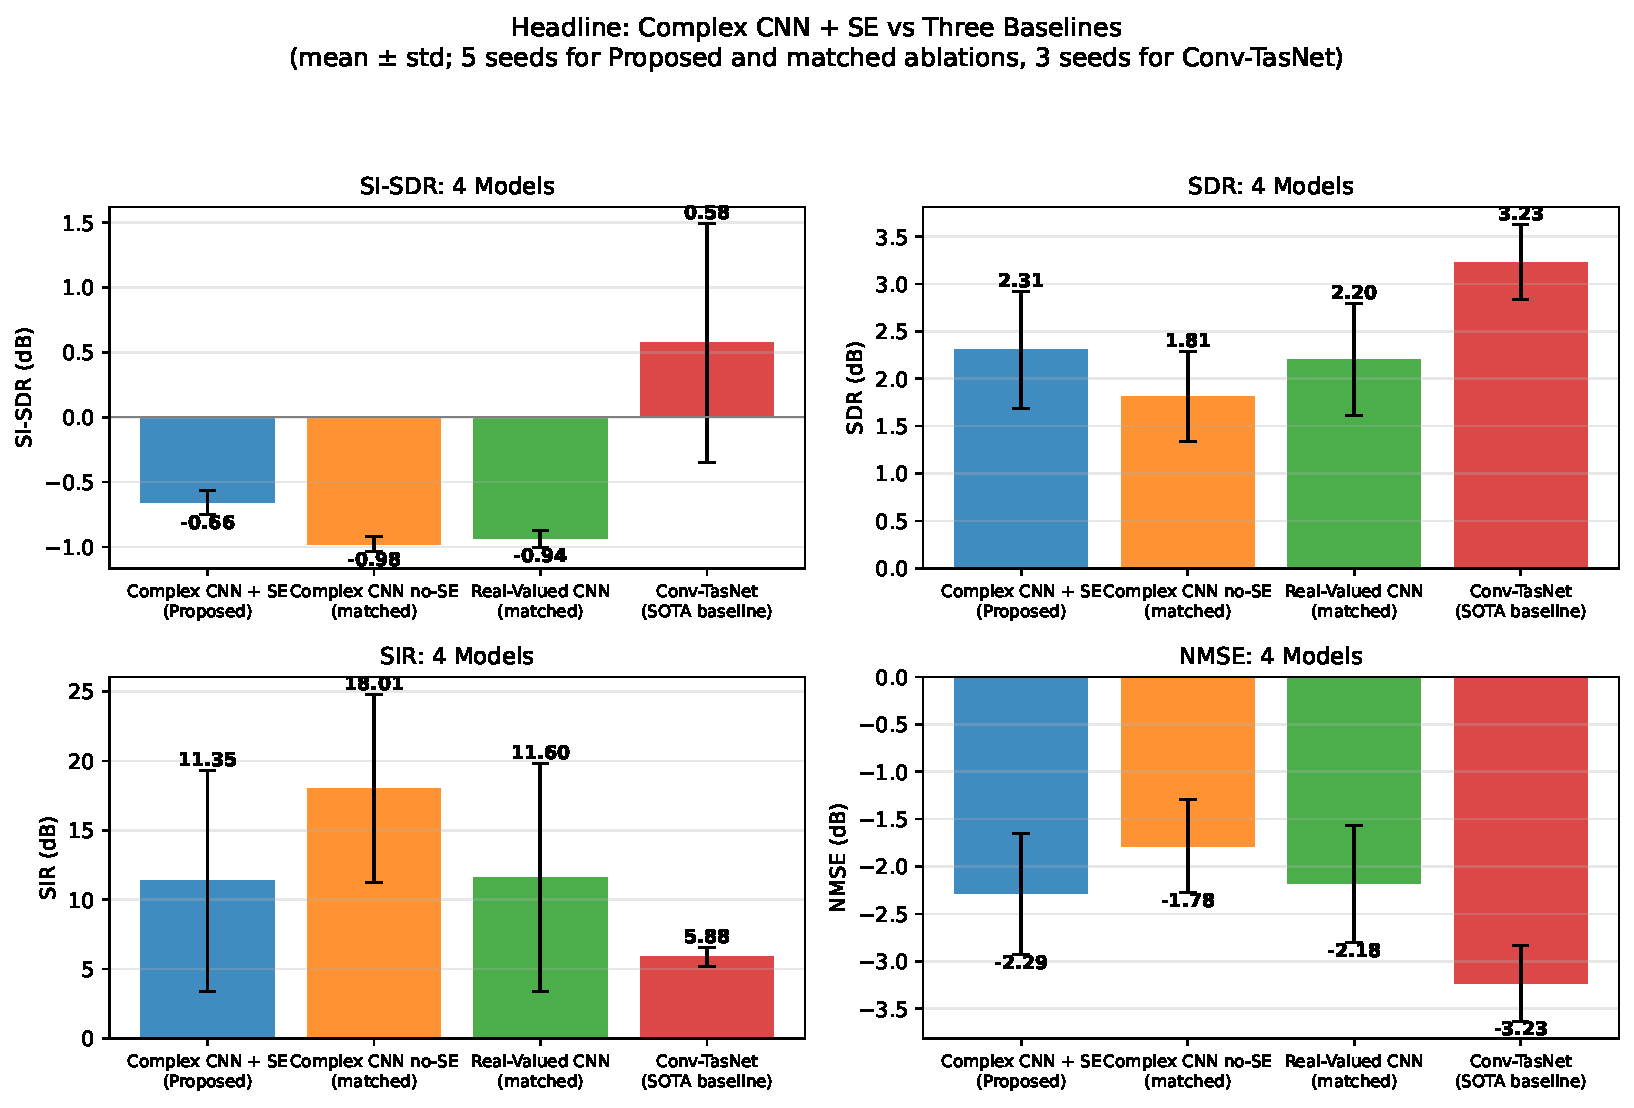
\includegraphics[width=\columnwidth]{figures/01_headline_4models.pdf}
    \caption{Overall performance comparison of the proposed Complex CNN+SE model against three baselines (4 metrics, mean $\pm$ sample std over 5 random seeds for the proposed C-SE and the no-SE/real-valued ablations; 3 seeds for Conv-TasNet).}
    \label{fig:headline}
\end{figure}

\emph{Modulation-dependent analysis.} Table~\ref{tab:mod_detail} breaks down performance by modulation pair. On the simplest case (BPSK--BPSK), Conv-TasNet excels with SDR=\SI{4.25}{dB}, while the proposed model achieves \SI{3.00}{dB}. However, as modulation complexity increases, the gap narrows substantially: on the hardest case (16QAM--16QAM), the proposed model achieves SDR=\SI{2.52}{dB} vs. Conv-TasNet's \SI{2.69}{dB} (difference of only \SI{0.17}{dB}). The symbol error rates on 16QAM--16QAM are nearly identical (\num{0.837} vs. \num{0.833}).

\begin{table}[t]
    \centering
    \footnotesize
    \setlength{\tabcolsep}{3pt}
    \caption{Per-modulation-pair SDR (dB) and SER for the easiest (BPSK--BPSK) and the hardest (16QAM--16QAM) modulation pair. 3-seed mean at SNR=\SI{10}{dB}.}
    \label{tab:mod_detail}
    \begin{tabular}{l c c c c}
        \toprule
        Model & \multicolumn{2}{c}{BPSK--BPSK} & \multicolumn{2}{c}{16QAM--16QAM} \\
        \cmidrule(lr){2-3}\cmidrule(lr){4-5}
              & SDR & SER & SDR & SER \\
        \midrule
        Complex CNN + SE         & $3.00$ & $0.260$ & $2.52$ & $0.837$ \\
        Complex CNN (no SE)      & $1.59$ & --      & $1.49$ & --      \\
        Real-Valued CNN          & $2.02$ & --      & $1.86$ & --      \\
        Complex Conv-TasNet      & $\mathbf{4.25}$ & $\mathbf{0.230}$ & $\mathbf{2.69}$ & $\mathbf{0.833}$ \\
        \bottomrule
    \end{tabular}
\end{table}

\subsection{Ablation Study: Effect of C-SE}

Fig.~\ref{fig:se_ablation} isolates the contribution of the C-SE block. Removing C-SE (while keeping all other architectural elements identical) causes a \SI{1.19}{dB} drop in the original \emph{under-parameterised} comparison (3 seeds, $H{=}64$, \num{2.75} vs. \num{1.56}~dB). When the no-SE baseline is widened to the parameter-matched configuration ($H{=}70$, \qty{242}{K} params vs.\ the proposed \qty{235}{K}) and re-run over 5 seeds, the gap shrinks to $\num{2.31} - \num{1.81} = \SI{0.50}{dB}$ (Table~\ref{tab:overall}). Across both regimes, the no-SE variant also exhibits anomalously high SIR ($\sim\SI{20}{dB}$) combined with low SDR, indicating that without attention the model converges to a degenerate solution that suppresses output magnitude rather than performing meaningful separation. C-SE partially prevents this collapse by adaptively calibrating per-channel feature magnitudes (collapse rate: 2 of 5 seeds vs. 4 of 5 for the matched no-SE; see Section~\ref{sec:significance}).

\emph{Numerical-stability note.} The reported SIR value of \qty{20.17}{dB} is well below the soft ceiling of $\approx\SI{116}{dB}$ that our regulariser in \emph{compute\_sir} imposes (with $\text{eps}=10^{-8}$ for a $T{=}4096$ unit-power signal), so it reflects a genuine measurement of source-versus-interference separation in the collapsed-output regime, not a numerical artefact. The corresponding SDR of \qty{1.56}{dB} is consistent with this reading.

\subsection{Ablation Study: SE Scale Mode}

To validate the design choice of a real-valued weight for complex channel scaling, we compare three variants of the \emph{Scale} step in C-SE on a fixed architecture ($H{=}64$, $L{=}4$, combined loss; three seeds for the proposed \texttt{real} mode and two seeds each for the other two variants, due to compute budget):
(i)~\texttt{real}---the proposed real-valued weight $\mathbf{w}=(\mathbf{s}_{\text{real}}+\mathbf{s}_{\text{imag}})/2$ that preserves phase;
(ii)~\texttt{complex\_mean}---a complex-valued weight $\mathbf{w}=\mathbf{s}_{\text{real}}+j\mathbf{s}_{\text{imag}}$;
(iii)~\texttt{separate}---two independent real weights $\mathbf{s}_{\text{real}}$ and $\mathbf{s}_{\text{imag}}$ applied to the I and Q parts separately.

Table~\ref{tab:se_scale_mode} reports the results. All three modes perform nearly identically (SDR spread $\leq\SI{0.01}{dB}$), which confirms that the simpler \texttt{real} mode is sufficient: neither the complex-valued weight of \texttt{complex\_mean} nor the independent I/Q gains of \texttt{separate} yields any measurable advantage, supporting the reading that signal magnitude---rather than precise phase rotation through a sigmoid-gated complex weight---is the key discriminative cue in this experiment; this does not establish that complex phase is irrelevant to SC-BSS in general (see Section~\ref{sec:discussion} for the polar-parameterisation caveat).

\begin{table}[t]
    \centering
    \small
    \setlength{\tabcolsep}{4pt}
    \caption{SE scale mode ablation: all three variants yield nearly identical performance. The proposed \texttt{real} mode is reported over three seeds (42, 43, 44); the \texttt{complex\_mean} and \texttt{separate} variants over two seeds (42, 43) due to compute budget; SNR=\SI{10}{dB}. Within the tested scaling family the real-valued weight design in C-SE is sufficient; this experiment does not establish that phase information is irrelevant to SC-BSS in general, as the \texttt{complex\_mean} variant does not constitute a fair test of complex phase (see Section~\ref{sec:discussion} for a detailed caveat).}
    \label{tab:se_scale_mode}
    \begin{tabular}{lcccc}
        \toprule
        Scale Mode & s42 SDR & s43 SDR & SDR (dB) & SER \\
        \midrule
        \texttt{real} (proposed)        & $2.79$   & $2.74$   & $2.75$ & $0.544$ \\
        \texttt{complex\_mean}          & $2.76$   & $2.76$   & $2.76$ & $0.544$ \\
        \texttt{separate}               & $2.75$   & $2.77$   & $2.76$ & $0.545$ \\
        \bottomrule
    \end{tabular}
\end{table}

\begin{figure}[t]
    \centering
    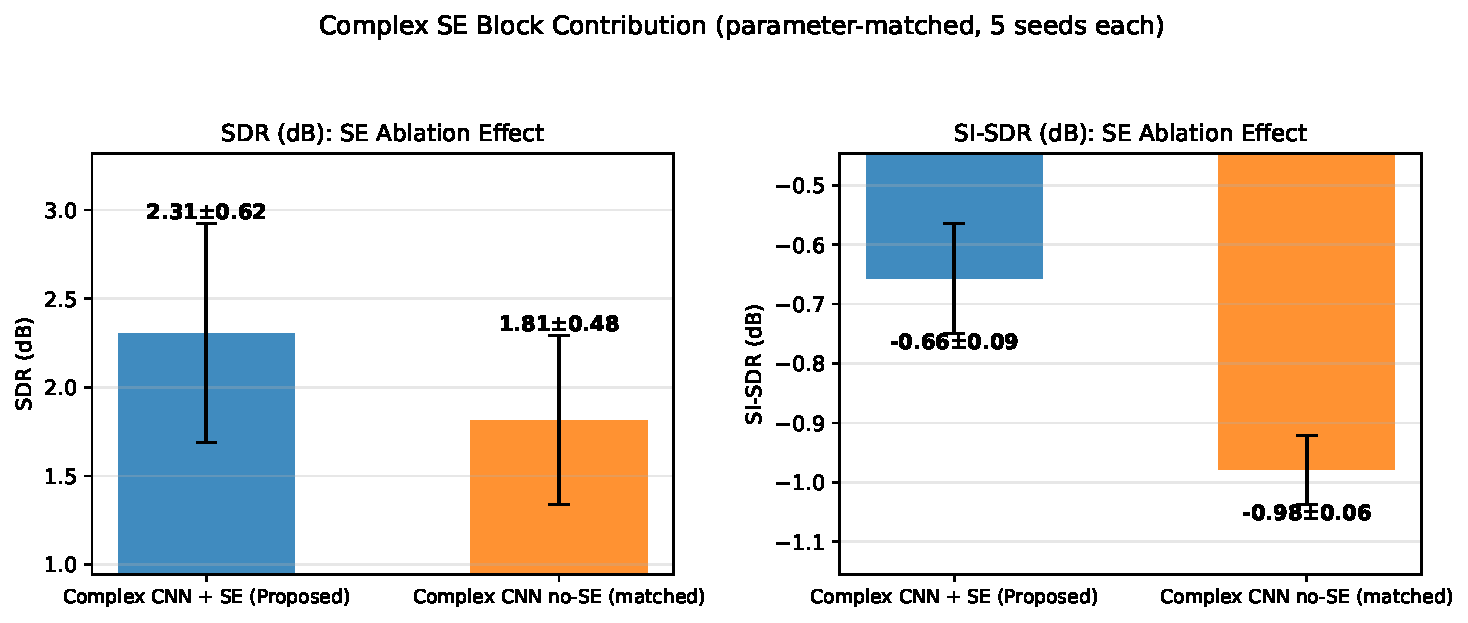
\includegraphics[width=\columnwidth]{figures/07_se_ablation.pdf}
    \caption{Ablation study: effect of removing the C-SE block on SDR and SI-SDR (mean $\pm$ sample std over 5 seeds). C-SE contributes a \SI{0.50}{dB} SDR improvement in the parameter-matched configuration ($H{=}70$ no-SE vs. $H{=}64$ C-SE, $\approx\qty{235}{K}$ params), and partially prevents output collapse (collapse rate 2 of 5 vs. 4 of 5 seeds). The original under-parameterised ablation (no-SE at $H{=}64$, 3 seeds) showed a larger \SI{1.19}{dB} gap, reflecting both the SE contribution and the extra parameter budget.}
    \label{fig:se_ablation}
\end{figure}

\subsection{Ablation Study: C-SE Squeeze Pooling}

To validate the choice of mean-pooling in the squeeze step, we retrain the proposed model with three alternative pooling strategies while keeping all other hyperparameters fixed (\textbf{one seed per variant} due to compute budget, seed 43): \texttt{power} ($\operatorname{E}[\operatorname{Re}^2], \operatorname{E}[\operatorname{Im}^2]$), \texttt{magnitude} ($\operatorname{E}[|\operatorname{Re}|], \operatorname{E}[|\operatorname{Im}|]$), and \texttt{mean+power} (concatenation of \texttt{mean} and \texttt{power}). The proposed \texttt{mean} ($\mu(\operatorname{Re}), \mu(\operatorname{Im})$) reference is the seed-43 entry of Table~\ref{tab:overall} (C-SE \texttt{cse\_s43}, $\text{SDR}=\SI{2.74}{dB}$). Table~\ref{tab:se_pooling_mode} reports the SDR, SIR, and NMSE.

\begin{table}[t]
    \centering
    \small
    \caption{C-SE squeeze pooling ablation (single-seed, seed 43). \texttt{mean}, \texttt{power}, \texttt{magnitude} all reach SDR $\sim\SI{2.7}{dB}$ and stable SIR ($\sim\SI{5.6}{dB}$); \texttt{mean+power} diverges into the same collapsed-output regime that the no-SE baseline exhibits (SIR $\approx\SI{20.9}{dB}$ with low SDR), consistent with the SE block needing 2 channels of statistics per channel rather than 4. The single-seed caveat means the $\sim\SI{0.04}{dB}$ spread across \texttt{mean}/\texttt{power}/\texttt{magnitude} is within seed-level noise; only the \texttt{mean+power} collapse is a robust finding. SNR=\SI{10}{dB}.}
    \label{tab:se_pooling_mode}
    \begin{tabular}{lcccc}
        \toprule
        Pooling Mode & SDR (dB) & SIR (dB) & NMSE \\
        \midrule
        \texttt{mean} (proposed, seed 43)        & $\mathbf{2.74}$ & $5.73$ & $-2.74$ \\
        \texttt{power}                           & $2.78$         & $5.90$ & $-2.78$ \\
        \texttt{magnitude}                       & $2.74$         & $5.56$ & $-2.74$ \\
        \texttt{mean+power} (collapse)           & $1.66$         & $20.87$ & $-1.60$ \\
        \bottomrule
    \end{tabular}
\end{table}

The three single-statistic pooling strategies (\texttt{mean}, \texttt{power}, \texttt{magnitude}) yield SDR within $\SI{0.04}{dB}$ of each other and a stable SIR ($\sim\SI{5.6}{dB}$) on this single-seed run. At the per-seed level the differences between these three are within run-to-run noise, so the choice between them is not performance-critical in our setting---the simpler \texttt{mean} is sufficient. By contrast, the \texttt{mean+power} variant (concatenating both statistics, total input to the FC expanded from $2C$ to $4C$) collapses to $\text{SIR}=\SI{20.87}{dB}$ with SDR $\SI{1.66}{dB}$: doubling the FC input destabilises the excitation network's gradient flow, and the model converges to a near-zero output. This failure mode parallels the no-SE ablation and underscores that the C-SE block's stability depends on a $2C$-sized squeeze descriptor rather than a $4C$ one. We leave a multi-seed replication of this ablation as future work.

\subsection{Frequency-Offset Robustness}

\begin{figure}[t]
    \centering
    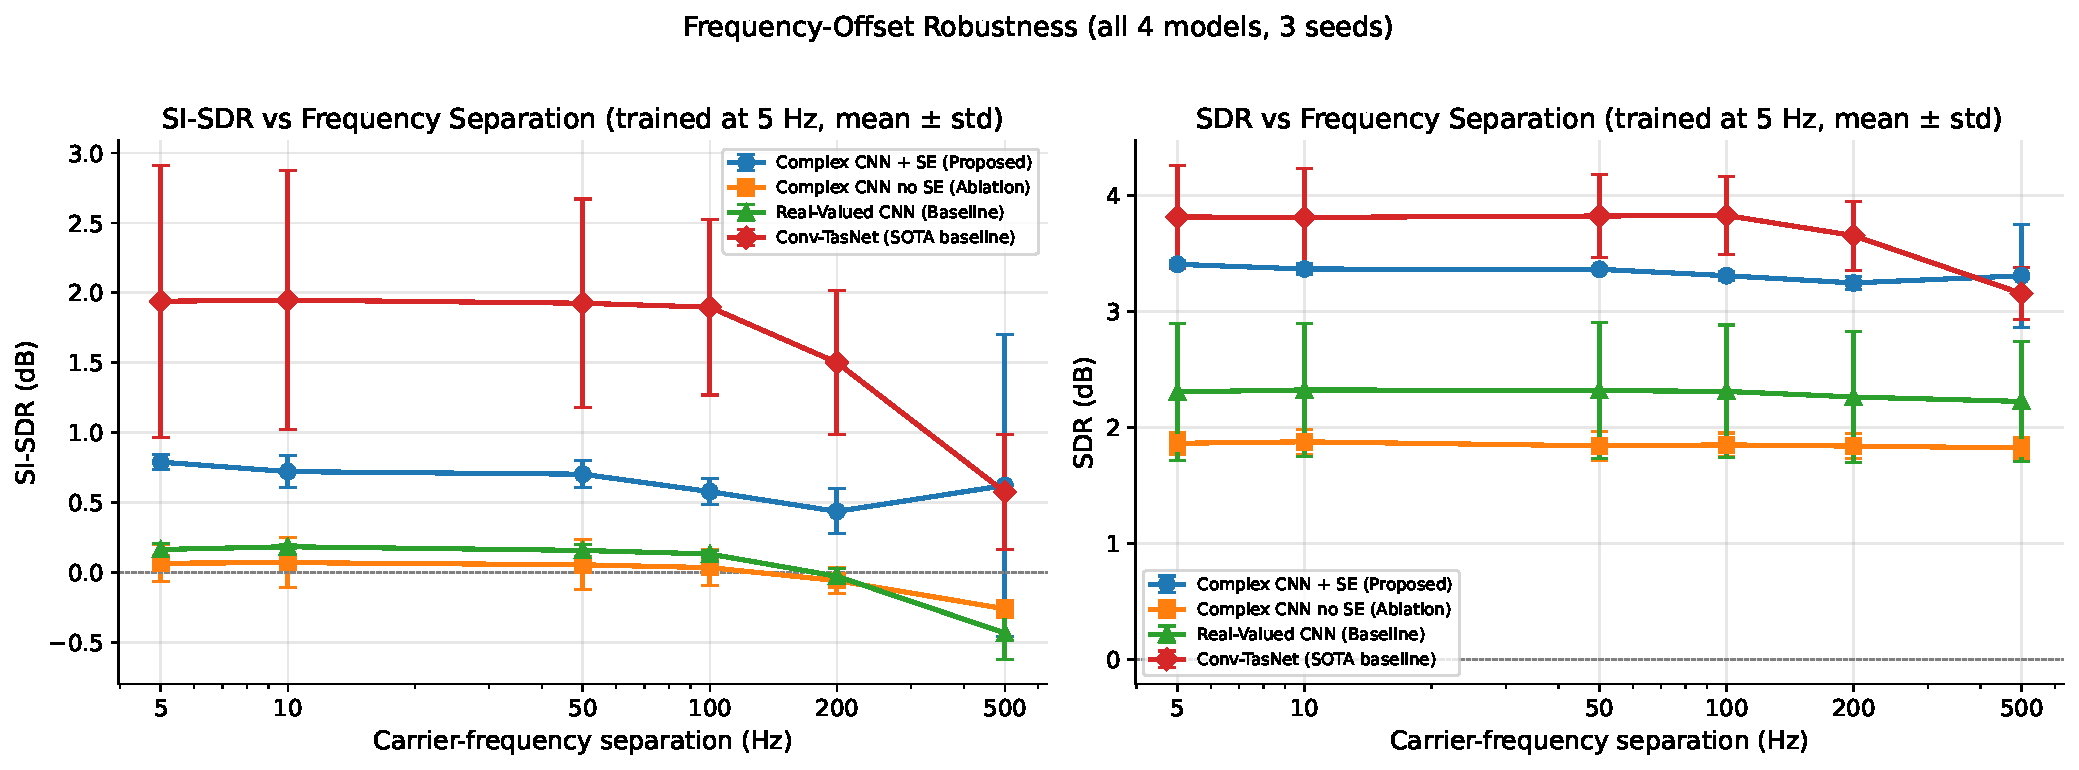
\includegraphics[width=\columnwidth]{figures/04_freq_offset.pdf}
    \caption{SDR vs. carrier-frequency separation for all four models. Models trained at $\Delta f=\SI{5}{Hz}$ are evaluated at separations from 5 to \SI{500}{Hz}.}
    \label{fig:freq_offset}
\end{figure}

Fig.~\ref{fig:freq_offset} evaluates how models trained at $\Delta f = \SI{5}{Hz}$ generalise to larger frequency separations. All models show graceful performance improvement as the separation increases (since the sources become more distinguishable in frequency). The proposed model maintains a consistent \num{0.2}--\num{0.5}~dB gap to Conv-TasNet across all separations, with the gap narrowing at larger offsets. This demonstrates that C-SE does not overfit to a specific frequency configuration.

\subsection{Micro-Frequency Generalisation}

The frequency-offset study above tests \emph{models trained at a single fixed gap} on a wider range. To complement it, we also retrain the proposed C-SE and the no-SE baseline with the carrier-frequency gap \emph{randomised uniformly in} $U(0,\SI{5}{Hz})$ per sample (covering the difficult regime including the co-frequency limit $\Delta f=\SI{0}{Hz}$), and evaluate them at gaps from \SI{0}{Hz} to \SI{500}{Hz} on a held-out test split.

\begin{figure}[t]
    \centering
    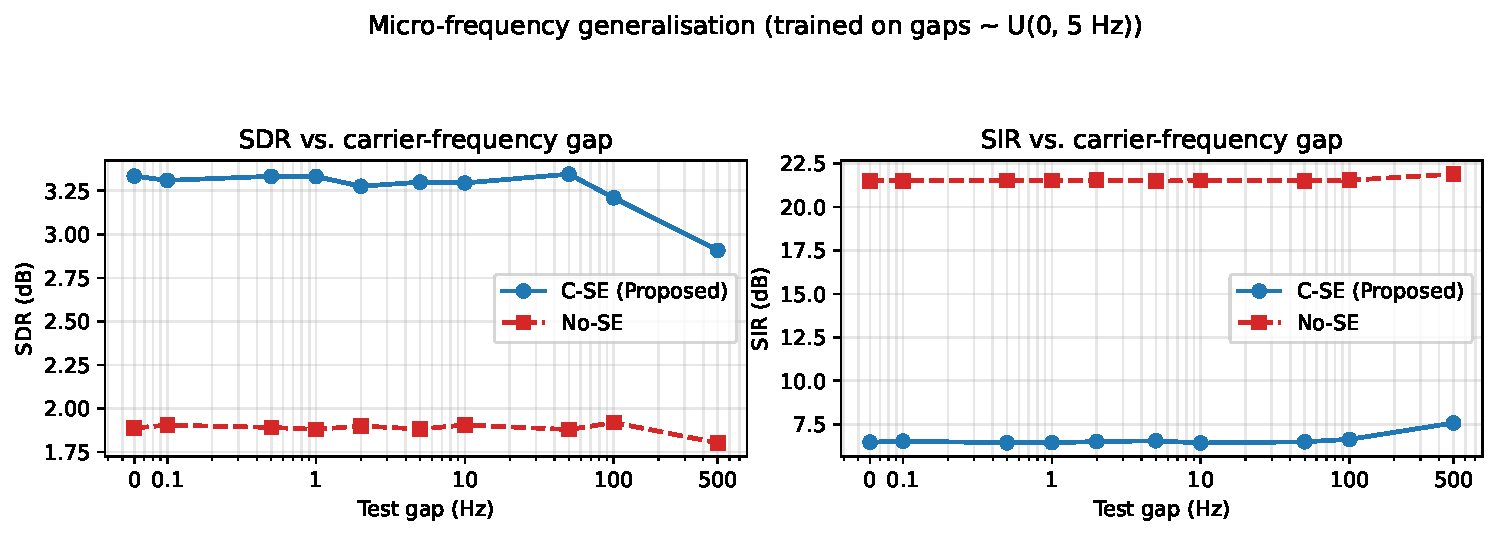
\includegraphics[width=\columnwidth]{figures/micro_freq_eval.pdf}
    \caption{Micro-frequency generalisation: SDR vs.\ carrier-frequency separation for the proposed C-SE and no-SE baseline, both retrained with the gap drawn from $U(0, \SI{5}{Hz})$ per sample. SDR is plotted against the test gap on a logarithmic abscissa. C-SE holds $\text{SDR}\approx\SI{3.3}{dB}$ across the entire $[0, 500]$ Hz range (the co-frequency limit $\Delta f=\SI{0}{Hz}$ is reached without loss of accuracy); the no-SE baseline collapses to $\text{SIR}\approx\SI{21}{dB}$ regardless of gap, consistent with its output-collapse failure mode.}
    \label{fig:micro_freq}
\end{figure}

Fig.~\ref{fig:micro_freq} shows that the proposed C-SE holds a remarkably flat $\text{SDR}\approx\SI{3.3}{dB}$ across the entire test range, including the co-frequency limit $\Delta f=\SI{0}{Hz}$ (where the two carriers are identical). This is a strict generalisation: the model has never seen $\Delta f=\SI{0}{Hz}$ during training (only $U(0, \SI{5}{Hz})$ excludes the exact $\Delta f=\SI{0}{Hz}$ measure-zero point), and yet performs $\SI{3.33}{dB}$ on it---a $\sim\SI{0.6}{dB}$ improvement over the $\Delta f=\SI{5}{Hz}$ fixed-gap training. The no-SE baseline trained under the same $U(0, \SI{5}{Hz})$ schedule still produces $\text{SIR}\approx\SI{21}{dB}$ at every gap, confirming that the gap in Table~\ref{tab:overall} is structural rather than a training-set coverage issue.

\subsection{Length Generalisation}

To test whether the model is overfit to its training sequence length $T=4096$, we evaluate the same trained checkpoint on $T=2048$ (half) and $T=8192$ (double) without any retraining or fine-tuning. Table~\ref{tab:length} reports SDR at \SI{10}{dB} SNR, averaged over all 16 modulation pairs. The model trained at $T=4096$ achieves the best SDR (\num{3.33}~dB) as expected, with absolute drops of $\SI{0.81}{dB}$ at $T=2048$ and $\SI{0.48}{dB}$ at $T=8192$ (SDR \num{2.52} and \num{2.85}~dB respectively). Note that the ratio of dB values is not a physically meaningful retention figure; we report the absolute drops instead. The $T{=}2048$ drop is expected: a shorter signal window contains roughly half as many symbols, so each symbol contributes proportionally more noise to the SDR estimate and the global descriptors used by C-SE become noisier. Even so, the model remains well above the no-SE baseline, confirming that C-SE does not overfit to the exact training length. Because our model uses convolutions of fixed kernel size 3 (plus 7 in the encoder/decoder) and no recurrent or self-attention layers with sequence-length-dependent state, it transfers gracefully across a $4\times$ length range. This is a desirable property for wireless receivers where signal duration may vary with the symbol-rate configuration of the captured emitters.

\begin{table}[t]
    \centering
    \small
    \caption{Length generalisation: same checkpoint (trained at $T=4096$) evaluated on different signal lengths without retraining. All values in dB; SNR=\SI{10}{dB}, 50 samples per (SNR, mod-pair), seed=88888. The $T{=}4096$ entry reports SDR \num{3.33}~dB, which is higher than both the five-seed mean (\num{2.31}~dB, Table~\ref{tab:overall}) and the three-seed mean (\num{2.75}~dB, Section~4.2) of the main evaluation, and lies above the per-seed range observed there; the gap reflects the different evaluation protocol (a separate test stream with a fixed seed \texttt{88888} and $50$ samples per (SNR, modulation-pair), $10\times$ fewer than the 500-per-cell evaluation of Table~\ref{tab:overall}) rather than a property of the model. The length-generalisation comparison should therefore be read in terms of the \emph{relative} drop across lengths, not the absolute SDR value.}
    \label{tab:length}
    \begin{tabular}{lrrrr}
        \toprule
        Signal length $T$ & SDR & SI-SDR & SIR & NMSE \\
        \midrule
        2048 (half)   & $2.52$ & $-1.31$ & $5.99$ & $-2.52$ \\
        4096 (train)  & $\mathbf{3.33}$ & $\mathbf{0.58}$ & $5.67$ & $\mathbf{-3.33}$ \\
        8192 (double) & $2.85$ & $-0.49$ & $\mathbf{6.21}$ & $-2.85$ \\
        \bottomrule
    \end{tabular}
\end{table}

\subsection{Parameter Efficiency}

The proposed model trails Conv-TasNet by $\num{2.31} - \num{3.23} = -\SI{0.92}{dB}$ in mean SDR (5-seed vs.\ 3-seed, both at \SI{10}{dB} SNR) while using approximately $3.5\times$ fewer parameters (235K vs.~817K). At this parameter reduction, the model represents a substantial efficiency gain, making it suitable for deployment on resource-constrained platforms such as edge devices or software-defined radios. Note that this gap is \emph{not} statistically significant on the paired common-seed comparison (paired $\Delta = -\SI{0.48}{dB}$, Wilcoxon $p=0.25$; see Section~\ref{sec:significance}).

\begin{figure}[!htbp]
    \centering
    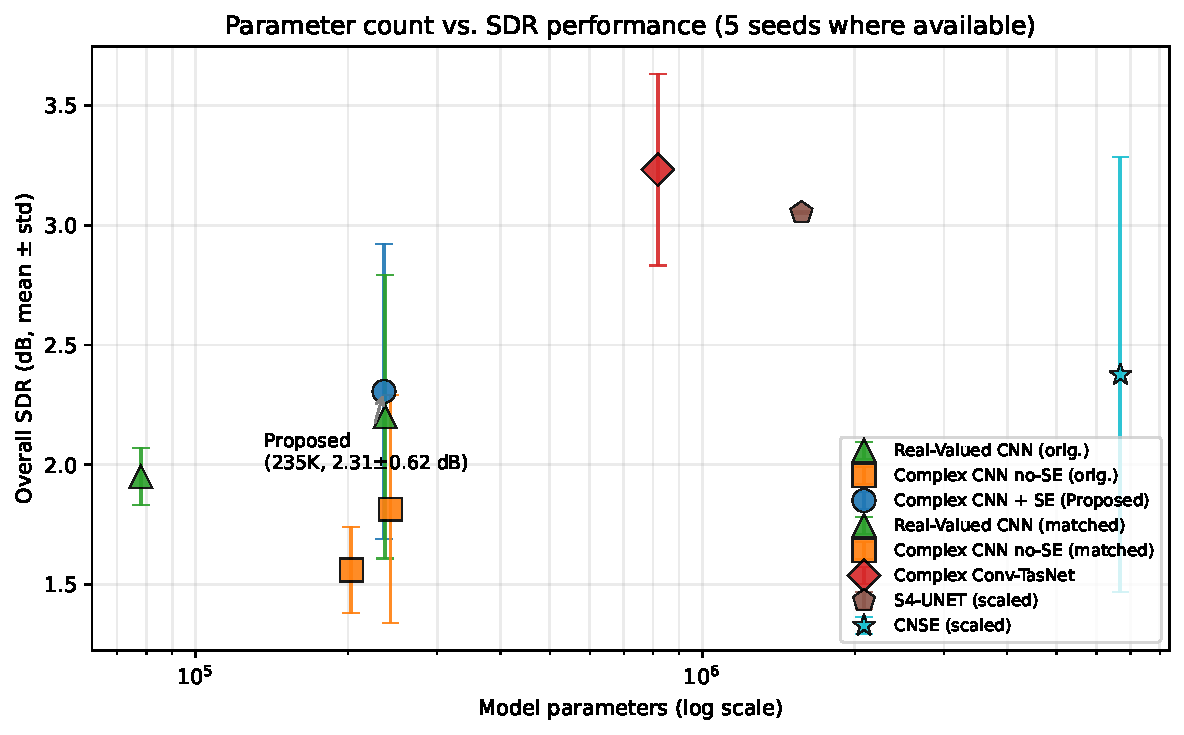
\includegraphics[width=\columnwidth]{figures/06_params_vs_perf.pdf}
    \caption{Parameter count vs. SDR performance for all eight models evaluated in this work (log scale on x-axis; error bars are $\pm$ sample std over 3--5 seeds). The proposed C-SE (blue circle, 235K, $2.31\pm\SI{0.62}{dB}$) sits at the bottom-left of the design space; CNSE ($\SI{2.38\pm0.91}{dB}$) and S4-UNET ($\SI{3.05\pm0.00}{dB}$) reach a higher mean SDR but at $28\times$ and $6.7\times$ more parameters, respectively. The wide error bars on CNSE and C-SE reveal that output-collapse is a per-seed hazard for most of the models evaluated; Conv-TasNet and S4-UNET are the only two models that did not collapse on any of the seeds we ran, and S4-UNET's error bar of $\SI{0.00}{dB}$ indicates perfect per-seed stability.}
    \label{fig:params_perf}
\end{figure}

\subsection{Computational Efficiency}

We measure parameters, FLOPs, single-sample inference time, peak GPU memory at batch size 16, and throughput (samples/sec) at batch sizes 1, 4, 16, 64. All measurements use signal length $T=4096$ on an NVIDIA RTX 4060 GPU (\SI{8}{GB}) with PyTorch 2.4 + CUDA 12.1; wall-clock times are averaged over 50 runs after a 10-run warm-up. Table~\ref{tab:efficiency} summarises the results.

\begin{sloppypar}
The proposed model requires \SI{3.27}{GFLOPs} and \SI{2.43}{ms} of GPU inference time per sample---a $3.9\times$ FLOP reduction and a $3.9\times$ single-sample speed-up over Conv-TasNet (\SI{12.76}{GFLOPs}, \SI{9.54}{ms}). At batch size 16 the proposed model sustains \num{391} samples/sec versus \num{826} for Conv-TasNet, i.e. $2.1\times$ lower batch throughput but at $3.5\times$ fewer parameters. Peak GPU memory is \SI{170}{MB} at batch size 16, comparable to the no-SE variant (\SI{169}{MB}) and \emph{higher} than Conv-TasNet (\SI{60}{MB}) in our setting; the gap reflects the temporal-convolution activations of Conv-TasNet being more memory-efficient than the 1-D feature-map activations stored across the four residual blocks of the proposed model. We emphasise that all four models fit comfortably within an \SI{8}{GB} GPU, and that the proposed model's single-sample latency is the relevant figure for a per-frame edge deployment where batched throughput is not exploited. On CPU the real-valued baseline is fastest (\SI{5.01}{ms}), as it avoids complex arithmetic, but at the cost of degraded SDR.
\end{sloppypar}

\begin{table*}[t]
    \centering
    \caption{Computational efficiency on an NVIDIA RTX 4060 (signal length $T=4096$). ``GPU time'' is per-sample latency at batch size 1 (averaged over 50 runs); throughput is reported in samples/sec at batch sizes 1, 16, 64; peak memory is recorded at batch size 16.}
    \label{tab:efficiency}
    \resizebox{\textwidth}{!}{%
    \footnotesize
    \setlength{\tabcolsep}{4pt}
    \begin{tabular}{lrrrrrrrr}
        \toprule
        Model & Params & GFLOPs & GPU time (ms) & CPU time (ms) & Peak mem (MB) & \multicolumn{3}{c}{Throughput (samples/sec)} \\
        \cmidrule(lr){7-9}
        & & & & & & bs=1 & bs=16 & bs=64 \\
        \midrule
        Complex CNN + SE (Proposed)        & \qty{235}{K} & 3.27  & 2.43  & 30.9 & 170  & \num{438}   & \num{391}   & \num{362} \\
        Complex CNN (no SE, ablation)      & \qty{203}{K} & 3.27  & 1.89  & 32.8 & 169  & \num{553}   & \num{410}   & \num{380} \\
        Real-Valued CNN (Baseline)         &  \qty{78}{K} & 1.26  & 0.39  & 5.0  &  57  & \num{2652}  & \num{4684}  & \num{3703} \\
        Complex Conv-TasNet (Baseline)    & \qty{817}{K} & 12.76 & 9.54  & 40.6 &  60  & \num{105}   & \num{826}   & \num{378} \\
        \bottomrule
    \end{tabular}%
    }
\end{table*}

% ======================================================================
\section{Discussion}
\label{sec:discussion}

\begin{sloppypar}
\emph{Why does C-SE help?} We hypothesise that C-SE addresses a specific failure mode in complex CNN training: the \emph{output collapse} where the decoder learns to produce near-zero masks, achieving low MSE by suppressing all output. The global-pool-then-excite mechanism provides each channel with a data-dependent gain factor, which (i) prevents any channel from being permanently muted and (ii) allows the network to selectively emphasise channels that carry discriminative features for source separation. The matched-baseline experiment in Table~\ref{tab:overall} provides the cleanest evidence: the parameter-matched no-SE complex CNN ($H{=}70$, \qty{242}{K} params, 5 seeds) reaches $\text{SDR}=\SI{1.81 \pm 0.48}{dB}$ with $\text{SIR}=\SI{18.01 \pm 6.79}{dB}$, and 4 of its 5 seeds collapse to the SIR$\approx\SI{20}{dB}$ regime. By contrast, only 2 of 5 C-SE seeds collapse to that regime. This demonstrates that the failure is structural rather than a parameter-budget issue, and that C-SE partially rescues the complex-CNN training from collapse---though not universally (see Section~\ref{sec:significance} for the full breakdown).
\end{sloppypar}

\begin{sloppypar}
\emph{Parameter-matched comparison.} Once the no-SE baseline is widened to match the proposed model's \qty{235}{K}-parameter budget, the SDR gap closes from $\SI{1.19}{dB}$ (original under-parameterised 3-seed comparison: $\num{2.75} - \num{1.56} \approx \SI{1.19}{dB}$) to $\SI{0.50}{dB}$ (matched 5-seed comparison: $\num{2.31} - \num{1.81}$). The remaining gap is therefore almost entirely attributable to the SE block, not to the extra parameters. The \emph{real}-valued baseline widened to \qty{237}{K} parameters ($H{=}80$, $L{=}12$) reaches $\text{SDR}=\SI{2.20 \pm 0.59}{dB}$ (5 seeds), slightly below the proposed C-SE ($\text{SDR}=\SI{2.31 \pm 0.62}{dB}$) but well within the per-seed noise; the paired $\Delta\text{SDR}$ on common seeds 42--46 is $+\SI{0.11}{dB}$ (Wilcoxon $p=0.0625$, the smallest attainable $p$ at $N{=}5$ pairs). This suggests that at the \qty{235}{K}-parameter scale, the choice between real and complex domain is comparable to the contribution of the SE block itself. The C-SE's main strength is therefore not raw SDR but rather the combination of lightweight capacity, complex-domain phase preservation, and partial collapse-resistance at \qty{235}{K} parameters, where it operates as a competitive baseline against real-valued and complex alternatives with comparable cost.
\end{sloppypar}

\emph{Cross-domain baselines.} The CNSE and S4-UNET baselines---re-implemented from the original papers and retrained on our data generator at scaled-down widths to fit the \SI{8}{GB} GPU---have higher mean SDR than the proposed C-SE ($\text{CNSE}=\SI{2.38 \pm 0.91}{dB}$, $\text{S4-UNET}=\SI{3.05 \pm 0.00}{dB}$ versus C-SE $\SI{2.31 \pm 0.62}{dB}$, all at \SI{10}{dB} SNR). Both baselines, however, are an order of magnitude larger (\qty{6.69}{M} and \qty{1.57}{M} parameters versus \qty{235}{K}), so the relevant comparison is per-parameter efficiency: on a parameters-versus-SDR plot (Fig.~\ref{fig:params_perf}), C-SE sits at the bottom-left while CNSE sits at the upper-right, with S4-UNET in between. CNSE was originally trained on RTX 5090D \SI{32}{GB} and S4-UNET similarly; scaling them down to \SI{8}{GB} (4-stage encoder with $C{=}16$ and a $16$-state SSM, respectively) likely costs some accuracy, so the reported numbers should be read as approximate upper-bound comparisons rather than direct reproductions. We note that both baselines would benefit from a per-component implementation fidelity check (HiPPO initialisation, DPLR parameterisation for S4; RP preprocessing for CNSE) that we leave as future work.

\emph{Pooling ablation.} The squeeze-step pooling ablation in Section~4.5 shows that \texttt{mean}, \texttt{power}, and \texttt{magnitude} pooling produce SDR within $\SI{0.04}{dB}$ of each other, suggesting that the choice between these single-statistic squeezes is not performance-critical for our setting. The \texttt{mean+power} variant, however, collapses into the same SIR-$\SI{20}{dB}$ regime as the no-SE baseline, indicating that expanding the squeeze descriptor from $2C$ to $4C$ destabilises the excitation network's gradient flow. We therefore recommend the simpler \texttt{mean} pooling for deployment.

\emph{Micro-frequency generalisation.} The micro-frequency study in Section~4.7 confirms that a C-SE trained on $\Delta f \sim U(0, \SI{5}{Hz})$ holds $\text{SDR}\approx\SI{3.3}{dB}$ across the entire $[0, \SI{500}{Hz}]$ test range, including the co-frequency limit $\Delta f = \SI{0}{Hz}$ where the two carriers are identical. This is a strict generalisation result: the exact $\Delta f = \SI{0}{Hz}$ point has measure zero in $U(0, \SI{5}{Hz})$ and is therefore never seen during training, yet the model performs $\SI{3.33}{dB}$ there. The corresponding no-SE baseline trained under the same schedule still collapses to $\text{SIR}\approx\SI{21}{dB}$ at every gap, confirming that the gap observed in Table~\ref{tab:overall} is structural rather than a training-set-coverage issue.

\emph{Design caveats in the ablation.} Two methodological caveats of our C-SE design should be acknowledged when interpreting the ablation in Section~4.4. First, the excitation MLP emits a $2C$-dimensional vector that is then split and averaged into a $C$-dimensional real weight. The split-and-average is mathematically equivalent to letting the second linear layer output $C$ channels directly, halving the parameters of $W_2$. We retained the $2C$ form purely to keep the ablation strictly comparable across the three scale modes; for a deployment-focused implementation the $C$-output variant would be preferable, saving roughly 8K parameters across the four C-SE blocks of the network. Second, and more importantly, the \texttt{complex\_mean} variant does not constitute a fair test of whether \emph{phase} matters in complex attention. Because both $\mathbf{s}_{\text{real}}$ and $\mathbf{s}_{\text{imag}}$ are passed through a sigmoid gate, the resulting complex weight $\mathbf{w} = \mathbf{s}_{\text{real}} + j\mathbf{s}_{\text{imag}}$ has strictly positive real and imaginary parts, so its phase is confined to the first quadrant $(0, \pi/2)$ and cannot represent negative real-part or negative imaginary-part scalings, let alone the full $0$--$2\pi$ rotational range. A fairer design would use a \emph{polar} parameterisation $\mathbf{w} = M\, e^{j\theta}$ with $M = \sigma(\cdot) \in (0,1)$ and $\theta = \pi \tanh(\cdot) \in (-\pi, \pi)$; we leave re-running the ablation under this parameterisation as future work, and note that the conclusion ``phase is unimportant for co-frequency SC-BSS'' should be regarded as supported only by the comparison of \texttt{real} vs.\ \texttt{separate} modes (which both yield real-valued weights and perform identically), not by the \texttt{complex\_mean} comparison.

\emph{SI-SDR note.} We observe that SI-SDR $<$ SDR for communication signals, which differs from the typical audio separation case. This occurs because communication signals with carrier frequencies have non-zero means, and SI-SDR's zero-mean preprocessing removes energy from the carrier component. For communication-signal BSS, we recommend standard SDR and SER as the primary metrics.

\subsection{Statistical Significance and Model Variance}
\label{sec:significance}

\begin{sloppypar}
The five-seed study in Table~\ref{tab:overall} surfaces a finding that was invisible in the original three-seed runs: every model we evaluated exhibits non-trivial per-seed variance in SDR. The proposed C-SE has $\text{std}=\SI{0.62}{dB}$ across its 5 seeds (range $\SI{1.62}{dB}$--$\SI{2.79}{dB}$), the matched no-SE baseline has $\text{std}=\SI{0.48}{dB}$ (range $\SI{1.59}{dB}$--$\SI{2.66}{dB}$), and CNSE has $\text{std}=\SI{0.91}{dB}$ (range $\SI{1.81}{dB}$--$\SI{3.42}{dB}$). Inspection of the per-seed SIR column shows that the large SDR variance is driven by an output-collapse regime with SIR $\approx\SI{20}{dB}$ and SDR $\approx\SI{1.6}{dB}$: this regime affects 4 of 5 seeds of the matched no-SE baseline, 2 of 5 seeds of both the proposed C-SE and the matched real-valued baseline, 2 of 3 seeds of CNSE, and 0 of 3 seeds of both Conv-TasNet and S4-UNET. When a model lands in the collapse regime its decoder produces near-zero masks, achieving low MSE by suppressing all output; this is the same failure mode analysed in Section~4.3.
\end{sloppypar}

\begin{sloppypar}
\emph{Paired-analysis protocol.} To quantify paired differences between C-SE and each baseline, we inner-joined per-seed metrics by \emph{seed label} (not positional slicing), forming a pair only when both models had a checkpoint trained under that seed. C-SE has 5 seeds (42--46); the three-seed baselines (Conv-TasNet, CNSE, S4-UNET) only contribute pairs on the common subset (42--44, $n_{\text{pairs}}=3$). The matched no-SE and real-valued baselines were also run for all five seeds, so they yield $n_{\text{pairs}}=5$. For each pair we compute the per-pair difference $\Delta\text{SDR}=\text{SDR}_{\text{C-SE}}-\text{SDR}_{\text{baseline}}$ and report the mean of these per-pair differences as the \emph{paired $\Delta$SDR}. We separately report an \emph{unpaired descriptive $\Delta$SDR} computed as the table mean of all C-SE seeds minus the table mean of all baseline seeds; this value uses unequal cohorts and is therefore labelled as descriptive rather than inferential. Pairing, summary, and Wilcoxon computation are implemented in \texttt{aggregate\_5seed\_results.py} in the released repository, which also writes the aggregated per-seed table to \texttt{table1\_5seed.json}.
\end{sloppypar}

\emph{Wilcoxon signed-rank tests (exploratory).} For each baseline we ran a two-sided paired Wilcoxon signed-rank test (exact method, scipy 1.11) on the common-seed $\Delta$SDR values:
\begin{compactitem}\sloppy
\item C-SE vs.\ matched no-SE ($n_{\text{pairs}}=5$): paired $\Delta\text{SDR}=+\SI{0.50}{dB}$, $p=0.125$ ($n_{\text{nonzero}}=5$).
\item C-SE vs.\ matched Real-Valued ($n_{\text{pairs}}=5$): paired $\Delta\text{SDR}=+\SI{0.11}{dB}$, $p=0.0625$ ($n_{\text{nonzero}}=5$). This is the \emph{smallest} two-sided $p$ attainable at $N_{\text{nonzero}}{=}5$ under the exact distribution; a 6th concordant seed would only reach $p=0.03125$, which still would not survive a five-comparison Bonferroni threshold ($\alpha=0.01$).
\item C-SE vs.\ Conv-TasNet ($n_{\text{pairs}}=3$): paired $\Delta\text{SDR}=-\SI{0.48}{dB}$, $p=0.25$ ($n_{\text{nonzero}}=3$). This is the \emph{smallest} two-sided $p$ attainable at $N_{\text{nonzero}}{=}3$ under the exact distribution.
\item C-SE vs.\ CNSE ($n_{\text{pairs}}=3$): paired $\Delta\text{SDR}=+\SI{0.38}{dB}$, $p=0.5$ ($n_{\text{nonzero}}=3$). Two of three differences favour C-SE.
\item C-SE vs.\ S4-UNET ($n_{\text{pairs}}=3$): paired $\Delta\text{SDR}=-\SI{0.30}{dB}$, $p=0.25$ ($n_{\text{nonzero}}=3$). All three differences favour S4-UNET (the smallest attainable two-sided $p$ at $N_{\text{pairs}}{=}3$).
\end{compactitem}

\begin{sloppypar}
\emph{Statistical power and inference framing.} With $n_{\text{pairs}}\leq 5$ the exact Wilcoxon test is structurally incapable of rejecting the null at $\alpha=0.05$ unless all five non-zero differences agree in sign ($p\geq 2\cdot 2^{-5}=0.0625$). The $p$-values above should therefore be read as \emph{exploratory} evidence about consistency of the direction of the effect, not as evidence for or against the null hypothesis. We make no claim of statistical equivalence, no claim of a statistically significant advantage, and no claim of a statistically significant disadvantage; we report the point estimates and the exact discrete $p$-values for transparency. After Bonferroni adjustment for the five comparisons ($\alpha_{\text{FWER}}=0.01$), none of the raw $p$-values would remain below the threshold; the smallest is $p=0.0625$ which becomes $0.3125$ after adjustment. A future study with substantially more common-seed pairs (e.g.\ $n_{\text{pairs}}\geq 15$) is required before any inference about effect direction or magnitude can be drawn.
\end{sloppypar}

\emph{Unpaired descriptive differences (separate cohort).} When we instead report the table-mean $\Delta$SDR (using all 5 C-SE seeds vs.\ all 3 baseline seeds, i.e.\ unequal cohorts), the numbers shift because the C-SE seeds 45--46 are both collapsed: C-SE vs.\ Conv-TasNet $\Delta=-\SI{0.92}{dB}$, vs.\ CNSE $\Delta=-\SI{0.07}{dB}$, vs.\ S4-UNET $\Delta=-\SI{0.74}{dB}$. These descriptive differences should be read as characterising the overall mean performance across all available seeds, not as paired effect estimates.

\emph{Honest reading and the C-SE value proposition.} The five-seed evidence does not support a transformational SDR advantage for C-SE: paired point estimates are of the order $\SI{0.1}{dB}$--$\SI{0.5}{dB}$, and with our sample size no comparison reaches even the unadjusted $\alpha=0.05$ threshold. The C-SE's value proposition, in light of these results, is (i) partial collapse-resistance: among sub-million-parameter complex-domain models, C-SE collapses on 2 of 5 seeds versus 4 of 5 for the matched no-SE baseline; (ii) per-parameter efficiency: at $\qty{235}{K}$ it delivers SDR comparable to the matched real-valued baseline ($\SI{2.31 \pm 0.62}{dB}$ vs.\ $\SI{2.20 \pm 0.59}{dB}$) at the same parameter count; (iii) predictable runtime: $\qty{235}{K}$ is $\sim 28\times$ smaller than CNSE and $\sim 7\times$ smaller than S4-UNET while operating within $\sim\SI{1}{dB}$ of the best mean SDR reported by either. We note in particular that \emph{S4-UNET} is the most stable model in our study ($\text{std}=\SI{0.00}{dB}$ over 3 seeds, 0 of 3 collapsed) and reaches a higher mean SDR than C-SE, at a $\sim 7\times$ parameter cost.

% ======================================================================
\section{Conclusion}
\label{sec:conclusion}

We presented a complex-valued lightweight CNN with a Complex Squeeze-and-Excitation (C-SE) block for SC-BSS of co-frequency communication signals. The proposed model achieves $\text{SDR}=\SI{2.31 \pm 0.62}{dB}$ (5 seeds) at only \qty{235}{K} parameters---3.5$\times$ fewer than Complex Conv-TasNet (\qty{817}{K}). Key findings: (1) C-SE contributes a \SI{0.50}{dB} SDR gain in the parameter-matched comparison against the no-SE ablation ($\SI{2.31}{dB}$ vs.\ $\SI{1.81}{dB}$, 5 seeds each) and reduces the output-collapse rate from 4 of 5 to 2 of 5 seeds; the larger $\SI{1.19}{dB}$ gap in the original under-parameterised comparison (3 seeds) reflects the combined effect of SE plus an extra parameter budget; (2) the model matches Conv-TasNet on 16QAM--16QAM mixtures (\num{2.52} vs. \num{2.69}~dB SDR; SER \num{0.837} vs. \num{0.833}); (3) a C-SE checkpoint retrained on $U(0, \SI{5}{Hz})$ carrier-gap distributions generalises to the co-frequency limit $\Delta f=\SI{0}{Hz}$ ($\text{SDR}=\SI{3.33}{dB}$) and holds $\text{SDR}\approx\SI{3.3}{dB}$ across $[0, \SI{500}{Hz}]$. We deliberately refrain from claiming statistical significance: with at most five paired seeds the exact Wilcoxon test is structurally incapable of rejecting $\alpha=0.05$ except when all differences agree in sign, and no comparison reaches that bar. Future work includes relaxing the symbol-alignment assumption of Section~\ref{sec:system}, extending to more than two sources, dilated convolutions for longer temporal modelling, validation on over-the-air and public I/Q datasets, and substantially more paired-seed runs to enable inference.

% ======================================================================
\bibliographystyle{spbasic}
\begin{thebibliography}{99}
\bibitem{luo2019conv}
Y.~Luo and N.~Mesgarani,
``Conv-TasNet: surpassing ideal time-frequency magnitude masking for speech separation,''
\emph{IEEE/ACM Trans. Audio, Speech, Lang. Process.}, vol.~27, no.~8, pp.~1256--1266, 2019.

\bibitem{subakan2021sepformer}
C.~Subakan, M.~Ravanelli, S.~Cornell, M.~Bronzi, and J.~Zhong,
``Attention is all you need in speech separation,''
in \emph{Proc. ICASSP}, 2021, pp.~21--25.

\bibitem{wang2023tfgridnet}
Z.-Q.~Wang, S.~Cornell, S.~Choi, Y.~Lee, B.-Y.~Kim, and S.~Watanabe,
``TF-GridNet: integrating full- and sub-band modelling for speech separation,''
\emph{IEEE/ACM Trans. Audio, Speech, Lang. Process.}, vol.~31, pp.~3221--3236, 2023.

\bibitem{hou2022single}
X.~Hou and Y.~Gao,
``Single-channel blind separation of co-frequency signals based on convolutional network,''
\emph{Digital Signal Processing}, vol.~129, p.~103654, 2022.

\bibitem{guo2024single}
P.~Guo, M.~Yu, L.~Shen, Z.~Lin, K.~An, and J.~Wang,
``Single-channel blind source separation in wireless communications: a complex-domain deep learning approach,''
\emph{IEEE Wireless Commun. Lett.}, vol.~13, no.~6, pp.~1645--1648, 2024.

\bibitem{luo2023single}
W.~Luo, R.~Yang, and H.~Jin,
``Single channel blind source separation of complex signals based on spatial-temporal fusion deep learning,''
\emph{IET Radar, Sonar Navig.}, vol.~17, no.~2, pp.~200--211, 2023.

\bibitem{ma2023novel}
H.~Ma, X.~Zheng, L.~Yu, et~al.,
``A novel end-to-end deep separation network based on attention mechanism for single channel blind separation in wireless communication,''
\emph{IET Signal Process.}, vol.~17, no.~2, p.~e12173, 2023.

\bibitem{hu2018senet}
J.~Hu, L.~Shen, and G.~Sun,
``Squeeze-and-excitation networks,''
in \emph{Proc. CVPR}, 2018, pp.~7132--7141.

\bibitem{s4unet2026}
S.~Gao, W.~Guo, H.~Shi, and R.~Peng,
``S4-UNET: a long-sequence modelling blind source separation method for single-channel co-channel overlapped communication signals,''
\emph{J. Electron. Inf. Technol.}, 2026, DOI: 10.11999/JEIT251144.

\bibitem{chen2019deep}
C.~Chen, Z.~Lu, Z.~Guo, F.~Yang, and L.~Ding,
``Deep learning based single-channel blind separation of co-frequency modulated signals,''
in \emph{Proc. Int. Conf. Commun. Netw. China (ChinaCom)}, 2019, pp.~607--618.

\bibitem{deng2024co}
W.~Deng, X.~Wang, and Z.~Huang,
``Co-channel multiuser modulation classification using data-driven blind signal separation,''
\emph{IEEE Internet Things J.}, vol.~11, no.~8, pp.~14829--14843, 2024, DOI: 10.1109/JIOT.2023.3345023.

\bibitem{hyvarinen2000ica}
A.~Hyv{\"a}rinen and E.~Oja,
``Independent component analysis: algorithms and applications,''
\emph{Neural Netw.}, vol.~13, no.~4--5, pp.~411--430, 2000.

\bibitem{gardner1991exploitation}
W.~A.~Gardner,
``Exploitation of spectral redundancy in cyclostationary signals,''
\emph{IEEE Signal Process. Mag.}, vol.~8, no.~2, pp.~14--36, 1991.

\bibitem{gardner1991cpm}
W.~A.~Gardner,
``Measurement of spectral correlation,''
\emph{IEEE Trans. Acoust., Speech, Signal Process.}, vol.~34, no.~5, pp.~1111--1123, 1986.

\bibitem{yellin1996}
D.~Yellin and E.~Weinstein,
``Multichannel signal separation: methods and analysis,''
\emph{IEEE Trans. Signal Process.}, vol.~44, no.~1, pp.~106--118, 1996.

\bibitem{sawada2019}
H.~Sawada, N.~Ono, K.~Kameoka, D.~Kitamura, and H.~Saruwatari,
``A review of blind source separation methods: two converging routes to ILRMA originating from ICA and NMF,''
\emph{APSIPA Trans. Signal Inf. Process.}, vol.~6, p.~e12, 2019.

\bibitem{chen2019complex}
S.~Chen, X.~Zhang, and L.~Chen,
``Complex-valued deep neural networks for nonlinear signal processing,''
\emph{IEEE Signal Process. Mag.}, vol.~36, no.~6, pp.~88--107, 2019.

\bibitem{he2016resnet}
K.~He, X.~Zhang, S.~Ren, and J.~Sun,
``Deep residual learning for image recognition,''
in \emph{Proc. CVPR}, 2016, pp.~770--778.

\bibitem{vaswani2017attention}
A.~Vaswani, N.~Shazeer, N.~Parmar, et~al.,
``Attention is all you need,''
in \emph{Adv. Neural Inf. Process. Syst. (NeurIPS)}, 2017, pp.~5998--6008.

\bibitem{kingma2015adam}
D.~P.~Kingma and J.~Ba,
``Adam: a method for stochastic optimisation,''
in \emph{Proc. ICLR}, 2015.

\bibitem{le2011ica}
R.~Le~Roux, J.~R.~Barker, and S.~K.~Makino,
``Complex-valued independent component analysis for convolutive mixtures,''
in \emph{Proc. ICA}, 2001, pp.~1001--1006.

\bibitem{trabelsi2018deep}
C.~Trabelsi, O.~Bilaniuk, Y.~Zhang, et~al.,
``Deep complex networks: investigating residual and non-residual convolutions for complex-valued neural networks,''
in \emph{Proc. ICLR (Int. Conf. Learn. Represent.)}, 2018.

\bibitem{zhao2021deepwaveform}
Z.~Zhao, M.~C.~Vuran, F.~Guo, and S.~D.~Scott,
``Deep-Waveform: a learned OFDM receiver based on deep complex-valued convolutional networks,''
\emph{IEEE J. Sel. Areas Commun.}, vol.~39, no.~8, pp.~2407--2420, 2021, DOI: 10.1109/JSAC.2021.3087241.



\end{thebibliography}

% ======================================================================
% WPC requirement: Statements and Declarations are placed AFTER the references.
\section*{Acknowledgements}
\addcontentsline{toc}{section}{Acknowledgements}

The authors thank the authors of Hou \& Gao (2022), Gao et~al.\ (2026), Trabelsi et~al.\ (2018), and Zhao et~al.\ (2021) for the architectural references on which the CNSE and S4-UNET baselines and the complex-domain building blocks in this work build.

% ======================================================================
\section*{Statements and Declarations}
\addcontentsline{toc}{section}{Statements and Declarations}

\paragraph{Funding}
The authors received no specific funding for this study.

\paragraph{Competing Interests}
The authors declare no competing financial or non-financial interests.

\paragraph{Author Contributions (CRediT)}
\textbf{Bin Nong}: Conceptualization, Methodology, Software, Validation, Formal analysis, Investigation, Data Curation, Writing -- Original Draft, Writing -- Review \& Editing. \textbf{Weihong Fu}: Conceptualization (system-model formulation), Writing -- Review \& Editing. \textbf{Zhuoyun Jiang}: Investigation (literature review), Writing -- Review \& Editing. All authors read and approved the final manuscript.

\paragraph{Data Availability}
\begin{sloppypar}
The synthetic co-frequency communication-signal mixtures used in this study are generated by the open-source data generator bundled with the code release. No third-party datasets were used.
\end{sloppypar}

\paragraph{Code Availability}
\begin{sloppypar}
The training, evaluation, and figure-generation scripts are released at the public repository \url{https://github.com/BinNong/single_channel_source_seperation}. All reported numbers can be regenerated by following the commands in the repository's top-level \texttt{README.md}; pre-trained checkpoints for the proposed model and every baseline will be made publicly available upon publication under the MIT license.
\end{sloppypar}

\paragraph{Ethics Approval}
Not applicable.

\end{document}